\documentclass[a4paper,12pt]{book}
\usepackage{graphicx}
\usepackage[export]{adjustbox}
\usepackage{subcaption}
\graphicspath{{Pics/}}
\usepackage{charter}
\usepackage{fancyhdr}
\usepackage{enumerate}
\usepackage{enumitem}
\usepackage{siunitx}
\usepackage{amssymb}
\usepackage{longtable}
\usepackage{multicol}
\usepackage{multirow}
\usepackage{hhline}
\usepackage{parskip}
\setlength{\parskip}{6pt}
\usepackage{ragged2e}
\usepackage{geometry} %margin
\geometry{left=2.1cm,right=2.1cm,top=3cm,bottom=3cm}
\usepackage{setspace}
\SetSinglespace{1.2}
\singlespacing
\renewcommand{\ttfamily}{\fontfamily{pcr}\selectfont}
%\renewcommand{\familydefault}{\rmdefault}

\usepackage[,table]{xcolor}
\definecolor{LightBlue}{cmyk}{0.16,0.03,0.04,0}
\definecolor{Title}{cmyk}{0.8,0.1,0,0.3}
\setlength{\arrayrulewidth}{0.3mm}
\setlength{\tabcolsep}{2pt}
\setlength{\headheight}{15pt}
\renewcommand{\arraystretch}{1}
\usepackage{tikz}
\usepackage{nicematrix}
\newcommand*\circled[1]{\tikz[baseline=(char.base)]{\node[shape=circle,draw,inner sep=1pt] (char) {#1};}}

\newcolumntype{s}{>{\columncolor{Title}\RaggedLeft} m{3.5em}} % columntype for chapter title
\newcolumntype{d}{>{\columncolor{LightBlue}\RaggedRight} m{\textwidth}} % columntype for code bloc
\newcolumntype{a}{>{\columncolor{LightBlue}\RaggedRight} m{0.96\textwidth}} % columntype for secondary code bloc

\usepackage{titlesec}
\usepackage[hidelinks]{hyperref}
\urlstyle{same}

\captionsetup[figure]{labelsep=period,font={bf}}
\captionsetup[table]{font={bf},labelsep=period}

\newcommand{\titlename}{}

\newcommand{\chaptertitle}[2]{ %reset chapter format
\vspace{-120pt}
\gdef\titlename{#1}
{
\SetSinglespace{1.1}
\singlespacing
\Huge\bfseries
\setlength{\tabcolsep}{8pt}
\renewcommand{\arraystretch}{1.5}
\begin{tabular}{s >{\RaggedRight}m{14.5em}}
\textcolor{white}{Chapter\newline\thechapter}&\textcolor{Title}{#2}
\end{tabular}
}
}

\newcommand{\partpic}[1]{%insert picture
    \tikz[remember picture,overlay] \node at (current page.center){\includegraphics[width=\paperwidth]{#1}};
}

\titleformat{\part} %reset part %format
{\huge\bfseries} % format
{} % label
{0em} % sep
{\Centering} % before-code

\titleformat{\chapter} %reset chapter %format
{\huge\bfseries} % format
{} % label
{0em} % sep
{\Centering} % before-code
\titlespacing{\chapter}{0pt}{0pt}{0pt}

\titleformat{\section} %reset section %format
{\Large\bfseries} % format
{\textcolor{Title}{\thesection}} % label
{0.5em} % sep
{\color{Title}} % before-code
\titlespacing{\section}{0pt}{12pt}{6pt}

\titleformat{\subsection} %reset subsection %format
{\large\bfseries} % format
{\textcolor{Title}{\thesubsection}} % label
{0.5em} % sep
{\color{Title}} % before-code
\titlespacing{\subsection}{0pt}{8pt}{6pt}

\newenvironment{term}[1]{
    \textbf{#1}

    \leftskip 1em
    \parskip 0pt
}

\newenvironment{secterm}[1]{
    \textbf{#1}

    \leftskip 2em
    \parskip 0pt
}

\newenvironment{codebloc}{ %define code bloc style
    \ttfamily\footnotesize
    \renewcommand{\arraystretch}{1}
}

\newcommand{\note}[2][NOTE]{ %Note/Tips
\vspace{6pt}
\begin{tabular}{b{\textwidth}}
\hline
\fontfamily{phv}\selectfont \textbf{#1}\\
\leftskip 1em #2\\
\hline
\end{tabular}
}

\newcommand{\secnote}[2][NOTE]{ %Note/Tips
\vspace{6pt}
\begin{tabular}{b{0.93\textwidth}}
\hline
\fontfamily{phv}\selectfont \textbf{#1}\\
\leftskip 1em #2\\
\hline
\end{tabular}
}

\title{ESP32-C3 Wireless Adventure\par \Large A comprehensive guide to IoT}
\author{Espressif Systems}
\date{\today}

\pagestyle{fancy} % reset head&foot
\fancyhead{} % clear all header fields
\renewcommand\headrulewidth{0pt}
\fancyfoot{} % clear all footer fields
\setcounter{chapter}{5}

\begin{document}

\fancyfoot[LE]{\fontfamily{cmss}\selectfont{\textbf{\thepage} \ \textit{ESP32-C3 Wireless Adventure: A comprehensive guide to IoT}}}
\fancyfoot[RO]{\fontfamily{cmss}\selectfont{\textit{Chapter \thechapter. \titlename} \ \textbf{\thepage}}}

\chapter[Driver Development]{\chaptertitle{Driver Development}{Driver Development}}

\vspace{36pt}
In the last chapter, we introduced the functions and hardware components of an IoT product (the Smart Light). In this chapter, we will move on to its driver development. Among the four layers of the IoT architecture, the perception \& control layer is intended to control objects, for example to switch on/off lights, or to open/close a curtain. To control different objects, corresponding hardware drivers are required, such as LED drivers and motor control drivers. The perception \& control layer can be combined with cloud computing, data mining, fuzzy recognition, and other AI technologies on the upper layer, to analyse and process massive data and information, smartly control objects, and realise real-time control, precise management, and scientific decision-making.

\section{Driver Development Process}
To develop a sensor driver, it generally takes three steps: know about the sensor, develop a sensor driver, and test the driver.

\begin{term}{1. Know about the sensor.}
    By reading the sensor’s datasheet or other means, learn about the characteristics of the sensor including its type, communication interface (e.g., I2C, SPI), measurement cycle, working mode, power mode, etc.
\end{term}

\begin{term}{2. Develop a sensor driver.}
    The main purpose of developing a sensor driver is to control the behaviors of the sensor through the SoC’s peripheral interfaces.
\end{term}

\begin{term}{3. Test the driver.}
    Once the development is done, write test cases to examine whether the driver can read data and control the peripheral interface successfully.
\end{term}

It takes similar steps to develop a controller driver: know about the controller, develop a driver, and test the driver.

\begin{term}{1. Know about the controller.}
    By reading the controller’s datasheet, learn about the controller’s working principles, so as to select a suitable peripheral interface.
\end{term}

\begin{term}{2. Develop a driver.}
    Based on the peripheral interface selected before, develop corresponding driver APIs for other embedded software modules.
\end{term}

\begin{term}{3.	Test the driver.}
    Write test cases to examine whether each driver API can be called and operate as expected.
\end{term}

\section{ESP32-C3 Peripheral Applications}
The ESP32-C3 chip has rich peripheral interfaces, as shown in Figure 6.1. In this section, we will introduce the application scenarios of ESP32-C3 peripheral interfaces in terms of the perception \& control layer.

\begin{figure}[h!]
    \centering
    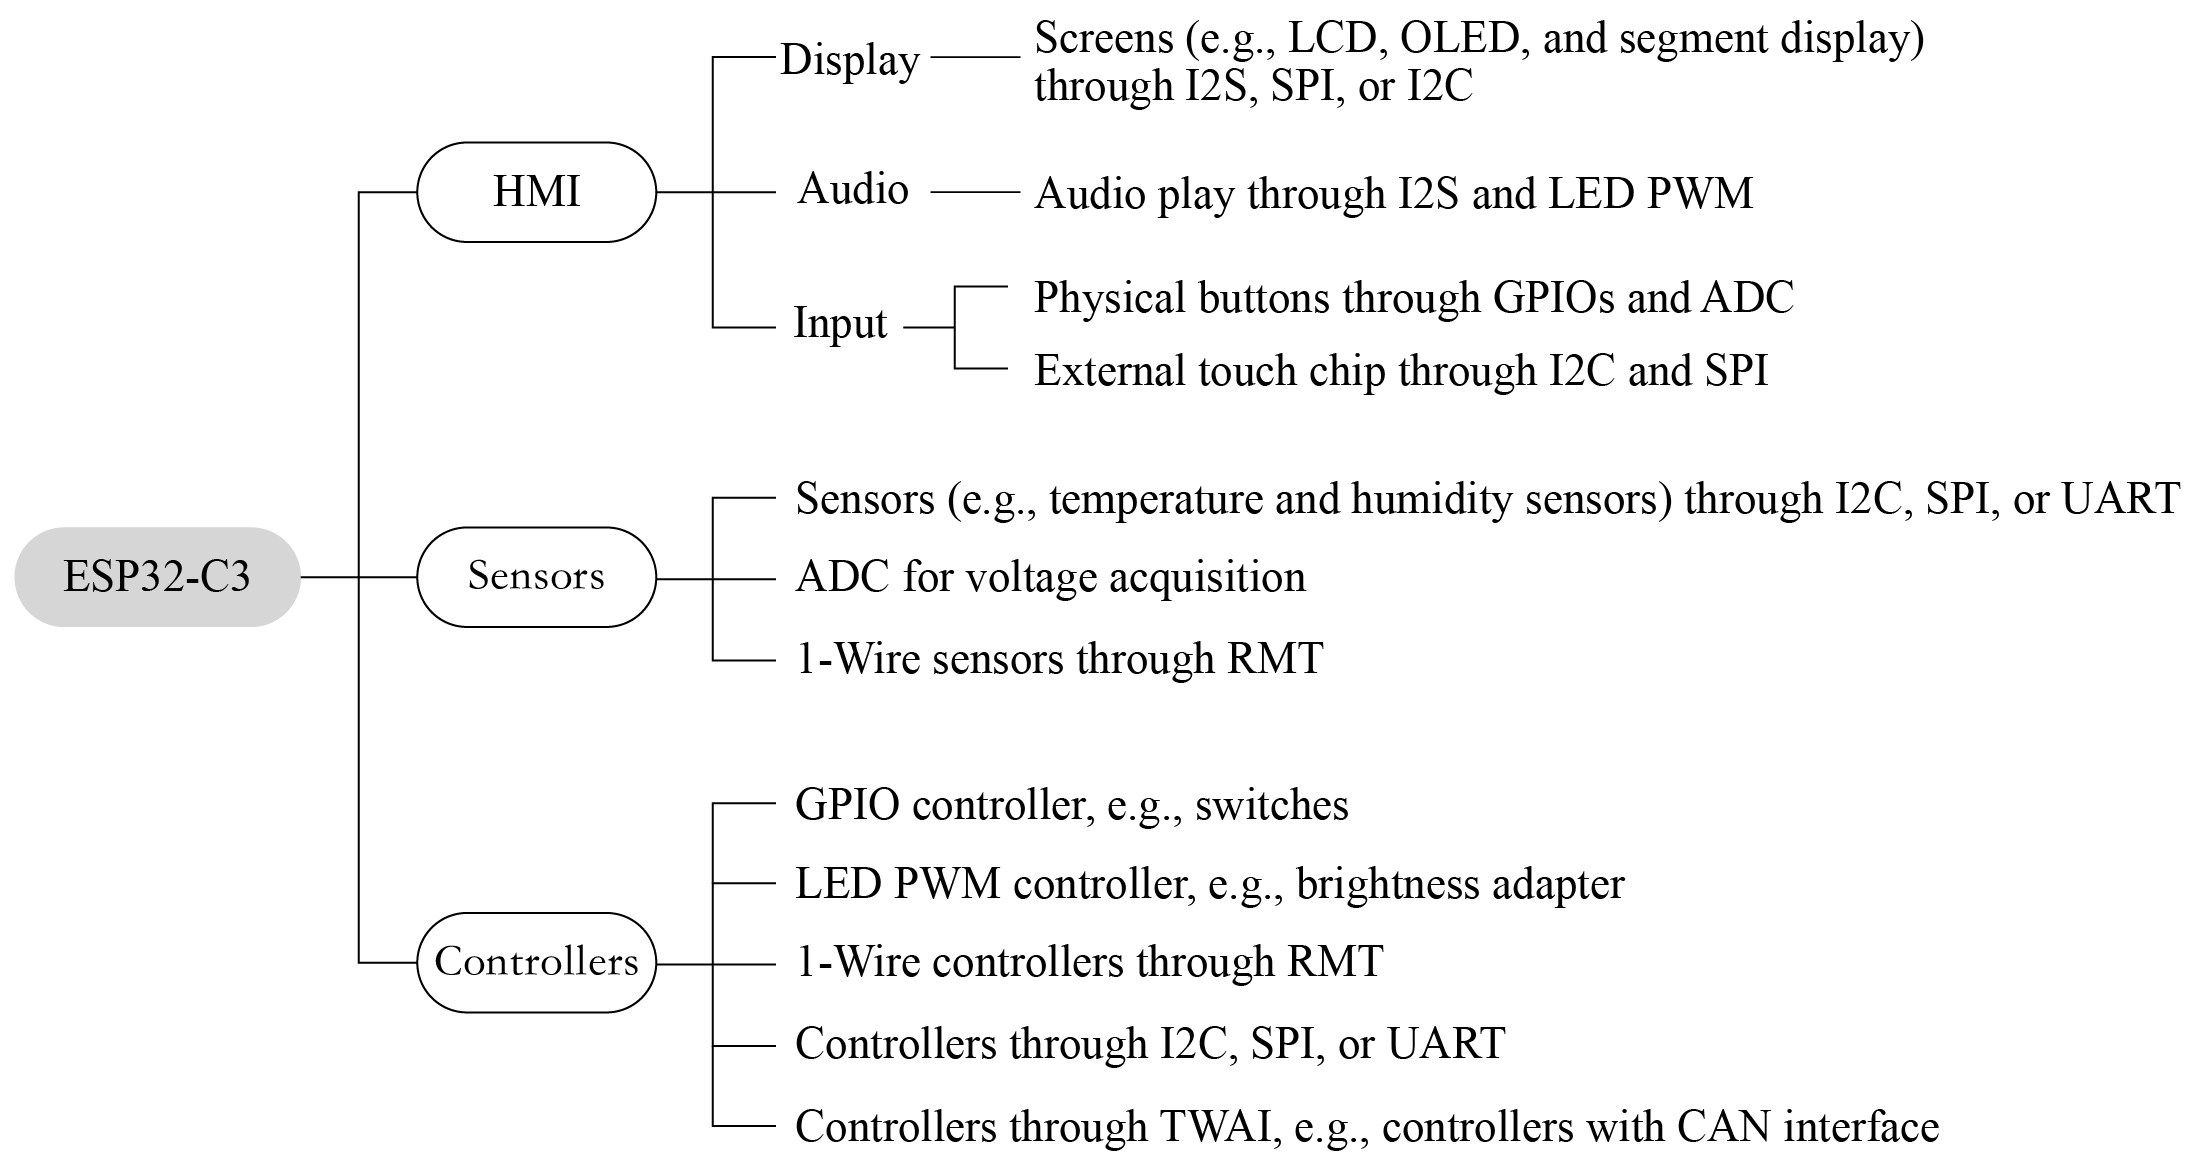
\includegraphics[width=0.9\textwidth]{D6Z/6-1}
    \caption{Peripheral applications of ESP32-C3}
\end{figure}

\begin{term}{Human Machine Interface (HMI)}
HMI products are digital devices composed of an input unit (e.g., touch screen and buttons) to receive commands and a display to show information, thus realising human machine interaction. According to their application scenarios, LCD displays, monochrome displays, and OLED displays can be connected through the SPI and I2C interfaces on ESP32-C3. GPIOs and ADC are used to read physical button inputs from users. Furthermore, capacitive touch pins of ESP32, ESP32-S2, and ESP32-S3 can be used for touch buttons, matrix buttons, linear sliders, 2D touch panels, and proximity sensing. These button and display related functions apply to smart door locks and other devices with screens. The I2S interface can be used to connect external audio codecs for devices with voice interaction features. The I2C interface can be used to drive digital tube displays or LED dot matrix displays, which are common for embedded applications. Compared with LCD displays, these displays use fewer GPIOs and less internal memory, and are easier to be implemented. They are more suitable for scenarios with simpler requirements such as timing, counting, and status display. 
\end{term}

\begin{term}{Sensors}
Simply speaking, sensors refer to devices and components that can convert various physical, chemical, and biological quantities in nature into measurable electrical signals. In this case, different types of sensors are needed. Sensors are the nerve endings of IoT and the core components for human beings to fully perceive nature. It is indispensable to deploy various sensors at a large scale for IoT development. We may use temperature and humidity sensors, inertial sensors, light sensors, air pressure sensors, gesture sensors, etc., depending on application scenarios. They need to be connected through different peripheral interfaces to function and collect data. As for ESP32-C3, I2C, SPI, and ADC are the common peripheral interfaces to drive sensors.

\vspace{6pt}
For your reference, drivers compatible with different types of sensors are provided in the \href{https://github.com/espressif/esp-iot-solution}{\texttt{espressif/esp-iot-solution}} repository on our GitHub.
\end{term}

\begin{term}{Controllers}
Controlling objects is an important function of the perception \& control layer. Control systems can be divided into two categories: the \textbf{open-loop system} and the \textbf{closed-loop system}. An open-loop control system, with no feedback mechanism, uses actuators to directly control objects. Its output signals have no influence or effect on other control actions within the system. But in closed-loop control systems, output is usually measured by sensors and fed back for comparison with the set point. The deviation between the actual output and the expected point is then used to automatically generate the next command. In smart home applications, common controlled objects include lighting, motors, and switches, which are mostly controlled by SoCs’ digital and analog signals. The LED PWM, GPIO, and ADC peripheral interfaces of ESP32-C3 can be used to tranmit the above signals.
\end{term}

\section{LED Driver Basics}
This section will introduce the basic knowledge of LED drivers, including color spaces in lighting, LED driver types, LED dimming methods, and PWM.

\subsection{Color Spaces}
Cyan, magenta, and yellow (CMY) are the three primary colors for painting. They mix with each other and generate a set of colors which constitue the CMY color space. We define the amount of magenta as the x axis, yellow as the y axis, and cyan as the z axis, thus creating a 3D space where each color has a unique position.

CMY is not the only color space. Computer monitors generally use the RGB (red, green, blue) color space, in which the amount of red, green, and blue are assigend as \textit{x}, \textit{y}, and \textit{z} axis. Another color space is HSV, which describes colors in terms of hue (\textit{x} axis), saturation (or chroma, \textit{y} axis) and value (or brightness, \textit{z} axis). The lighting industry commonly uses the HSL color space, which generates colors by changing hue, saturation, and lightness.

\subsubsection{1. RGB color space}
The RGB color space is the one we are most familiar with. As shown in Figure 6.2, this color space is represented by mixing the three primary colors to reproduce almost any color. It is the basic, hardware-oriented color space commonly used in image processing, and is relatively easy to understand. It uses a linear combination of three primary colors to represent a secondary color. The three primary components are highly correlated, so it is not visually intuitive when transitioning colors continuously. To adjust the color of an LED, you need to change the amount of all three primary colors.

\begin{figure}[h!]
    \centering
    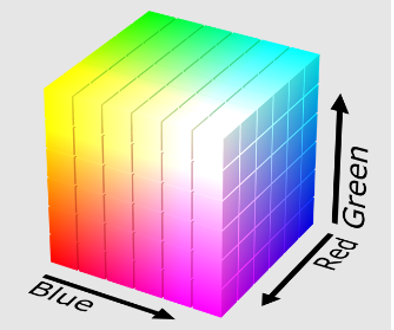
\includegraphics[width=0.4\textwidth]{D6Z/6-2}
    \caption{RGB color space}
\end{figure}

Images acquired in natural environments are easily affected by natural light, occlusion, and shadows. That is, they are sensitive to brightness. The amount of three primary colors in the RGB color space are closely related to brightness. So long as the brightness changes, the amount of all three colors will change accordingly. There is, however, no intuitive way to reflect this change. The human eye is not equally sensitive to the three colors. In monochrome vision, the human eye is least sensitive to red and most sensitive to blue. Due to this variation in sensitivity, the RGB color space is considered to have poor uniformity. The way the human eye perceives color similarities deviates greatly from the Euclidean distance in the RGB color space. Therefore, it is difficult for human beings to represent a color accurately by the amount of three primary colors.

\subsubsection{2. HSV color space}
The HSV color space is widely used in computers, as shown in Figure 6.3. Compared with the RGB color space, HSV is closer to the human perception of colors. It can intuitively represent the hue, saturation, and brightness value of colors for comparison.

\begin{figure}[h!]
    \centering
    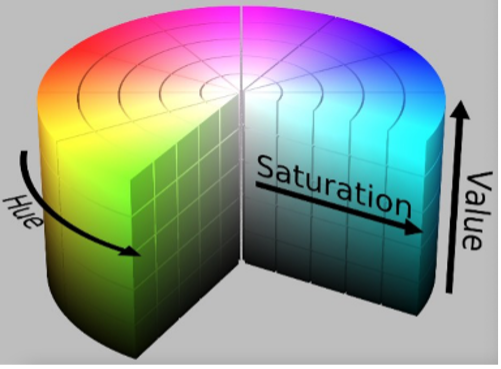
\includegraphics[width=0.35\textwidth]{D6Z/6-3}
    \caption{HSV color space}
\end{figure}

It is easier to track an object of a particular color in the HSV space than in the RGB space, and thus the HSV color space is often used to segment objects of a specified color. HSV space defines colors in terms of hue, saturation, and value (brightness).

Usually, the HSV color space is mapped to a cylinder. The cross section of the cylinder can be regarded as a polar coordinate system, in which the polar angle is interpreted as hue, the polar axis length interpreted as saturation, and the height of the cylinder axis as value. Hue is measured in angle and ranges from 0 to 360°, indicating the position of the spectral color. Figure 6.4 illustrates hue in the HSV color space.

\begin{figure}[h!]
    \centering
    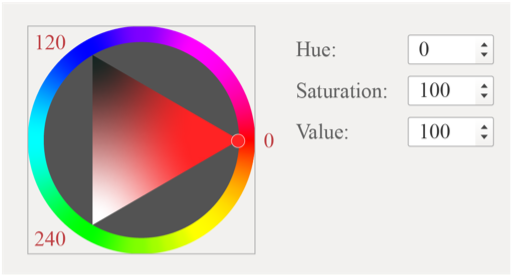
\includegraphics[width=0.45\textwidth]{D6Z/6-4}
    \caption{HSV color space – hue}
\end{figure}

In Figure 6.4, all the colors on the wheel are spectrum colors. Calculated counterclockwise from red, 0 represents red, 120° represents green, and 240° represents blue.

In the RGB color space, one color is determined by three values. For example, yellow is represented by (255,255,0). In the HSV color space, yellow is represented by only one value, i.e., Hue=60.

Figure 6.5 is the semi horizontal cross-section of the cylinder (Hue=60) and illustrates saturation and value in the HSV color space.

\begin{figure}[h!]
    \centering
    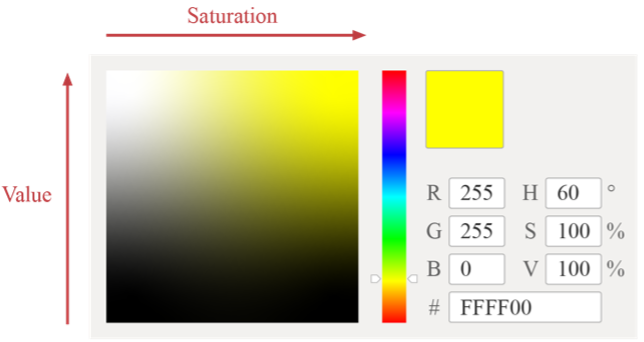
\includegraphics[width=0.5\textwidth]{D6Z/6-5}
    \caption{HSV color space – saturation and value}
\end{figure}

In Figure 6.5, the horizontal axis represents saturation, which indicates the deviation from the spectrum colors. It ranges from 0\% to 100\%, where 0 represents pure white. The higher the saturation, the darker the color, the closer to the spectrum color, and vice versa.

The vertical axis represents value, which indicates the brightness of the color in the HSV color space. Value ranges from 0\% to 100\%, where 0 represents plain black. The higher the value, the brighter the color.

\subsubsection{3. HSL color space}
The HSL color space is similar to the HSV color space. It also has three components: hue, saturation, and lightness. The difference lies in the last component. Lightness in HSL represents luminance. A lightness of 100 means white, whereas a lightness of 0 means black. Value in HSV represents brightness. A value of 100 equals spectrum color, whereas a value of 0 equals black. Figure 6.6 shows the HSL color space.

\begin{figure}[h!]
    \centering
    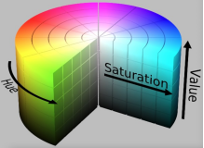
\includegraphics[width=0.4\textwidth]{D6Z/6-6}
    \caption{HSL color space}
\end{figure}

Figure 6.7 shows hue in the HSL color space, which represents the range of colors the human eye can perceive. They are distributed on a flat color wheel; each represented by a hue of 0 to 360°. The significance of hue is that we can change the color by rotating the color wheel without changing saturation or lightness.

\begin{figure}[h!]
    \Centering
    \begin{subfigure}{0.4\textwidth}
        \RaggedLeft
        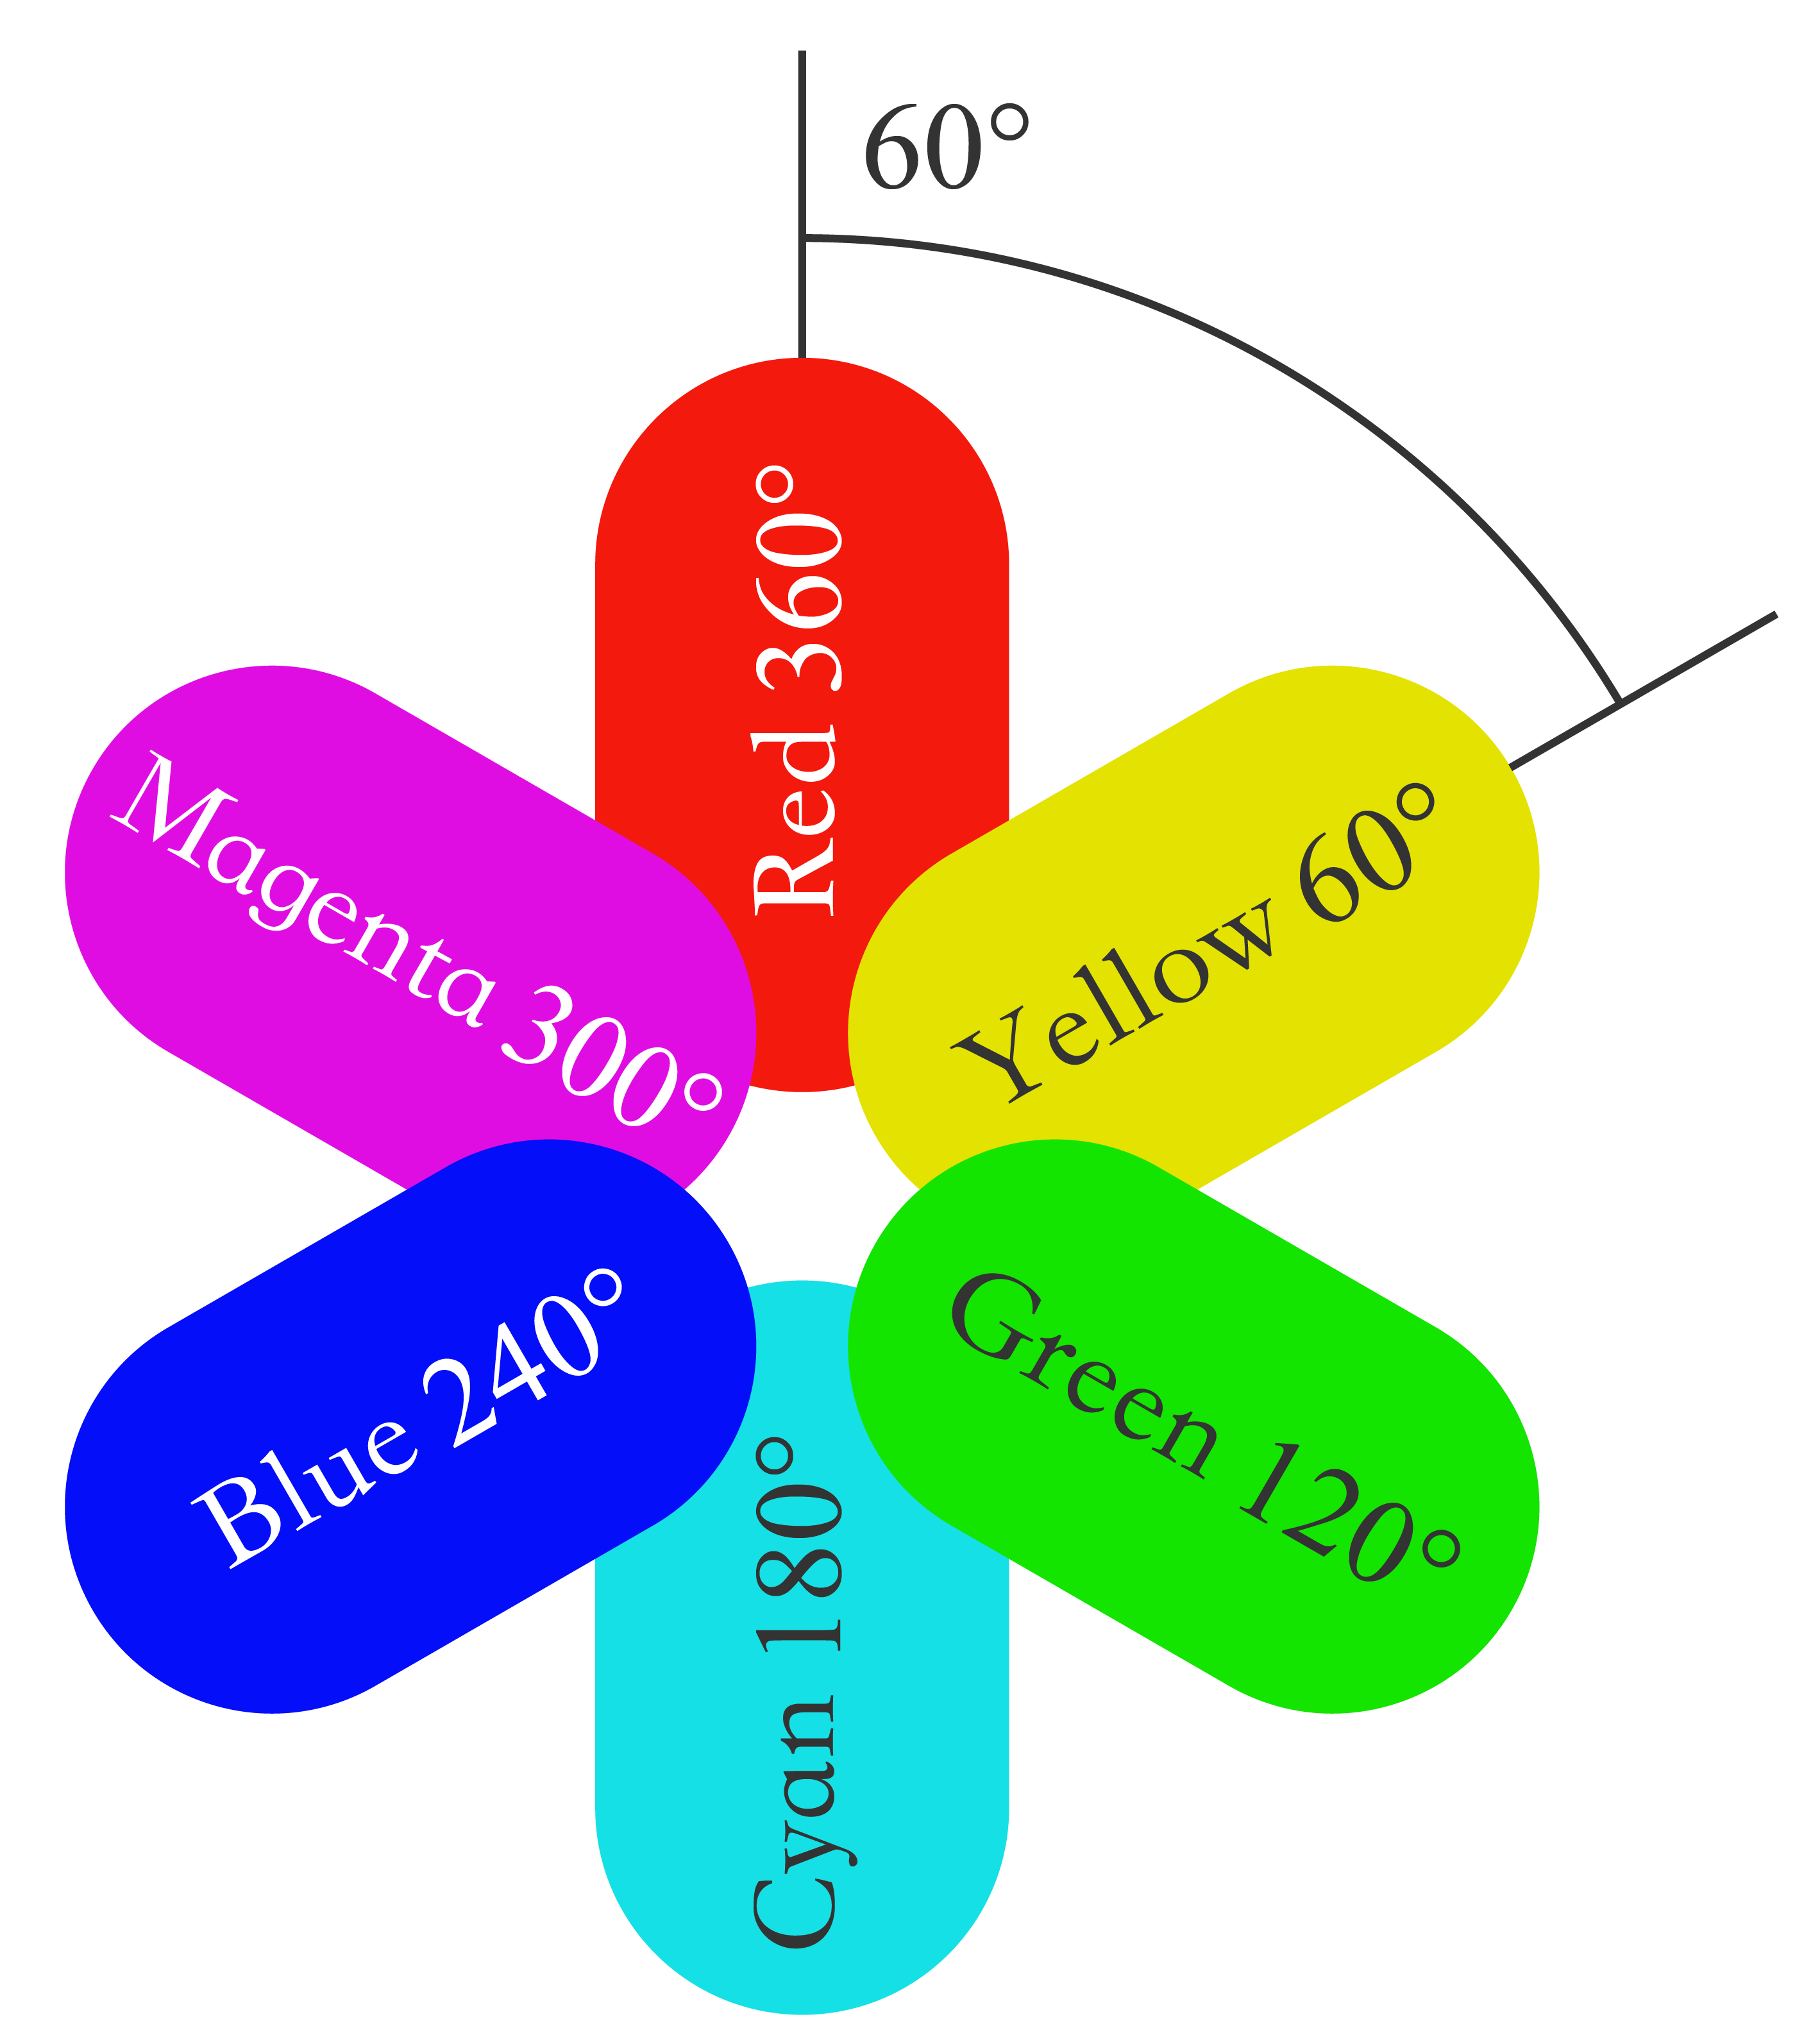
\includegraphics[height=0.8\textwidth]{D6Z/6-7a} 
    \end{subfigure}\hspace{1em}
    \begin{subfigure}{0.4\textwidth}
        \RaggedRight
        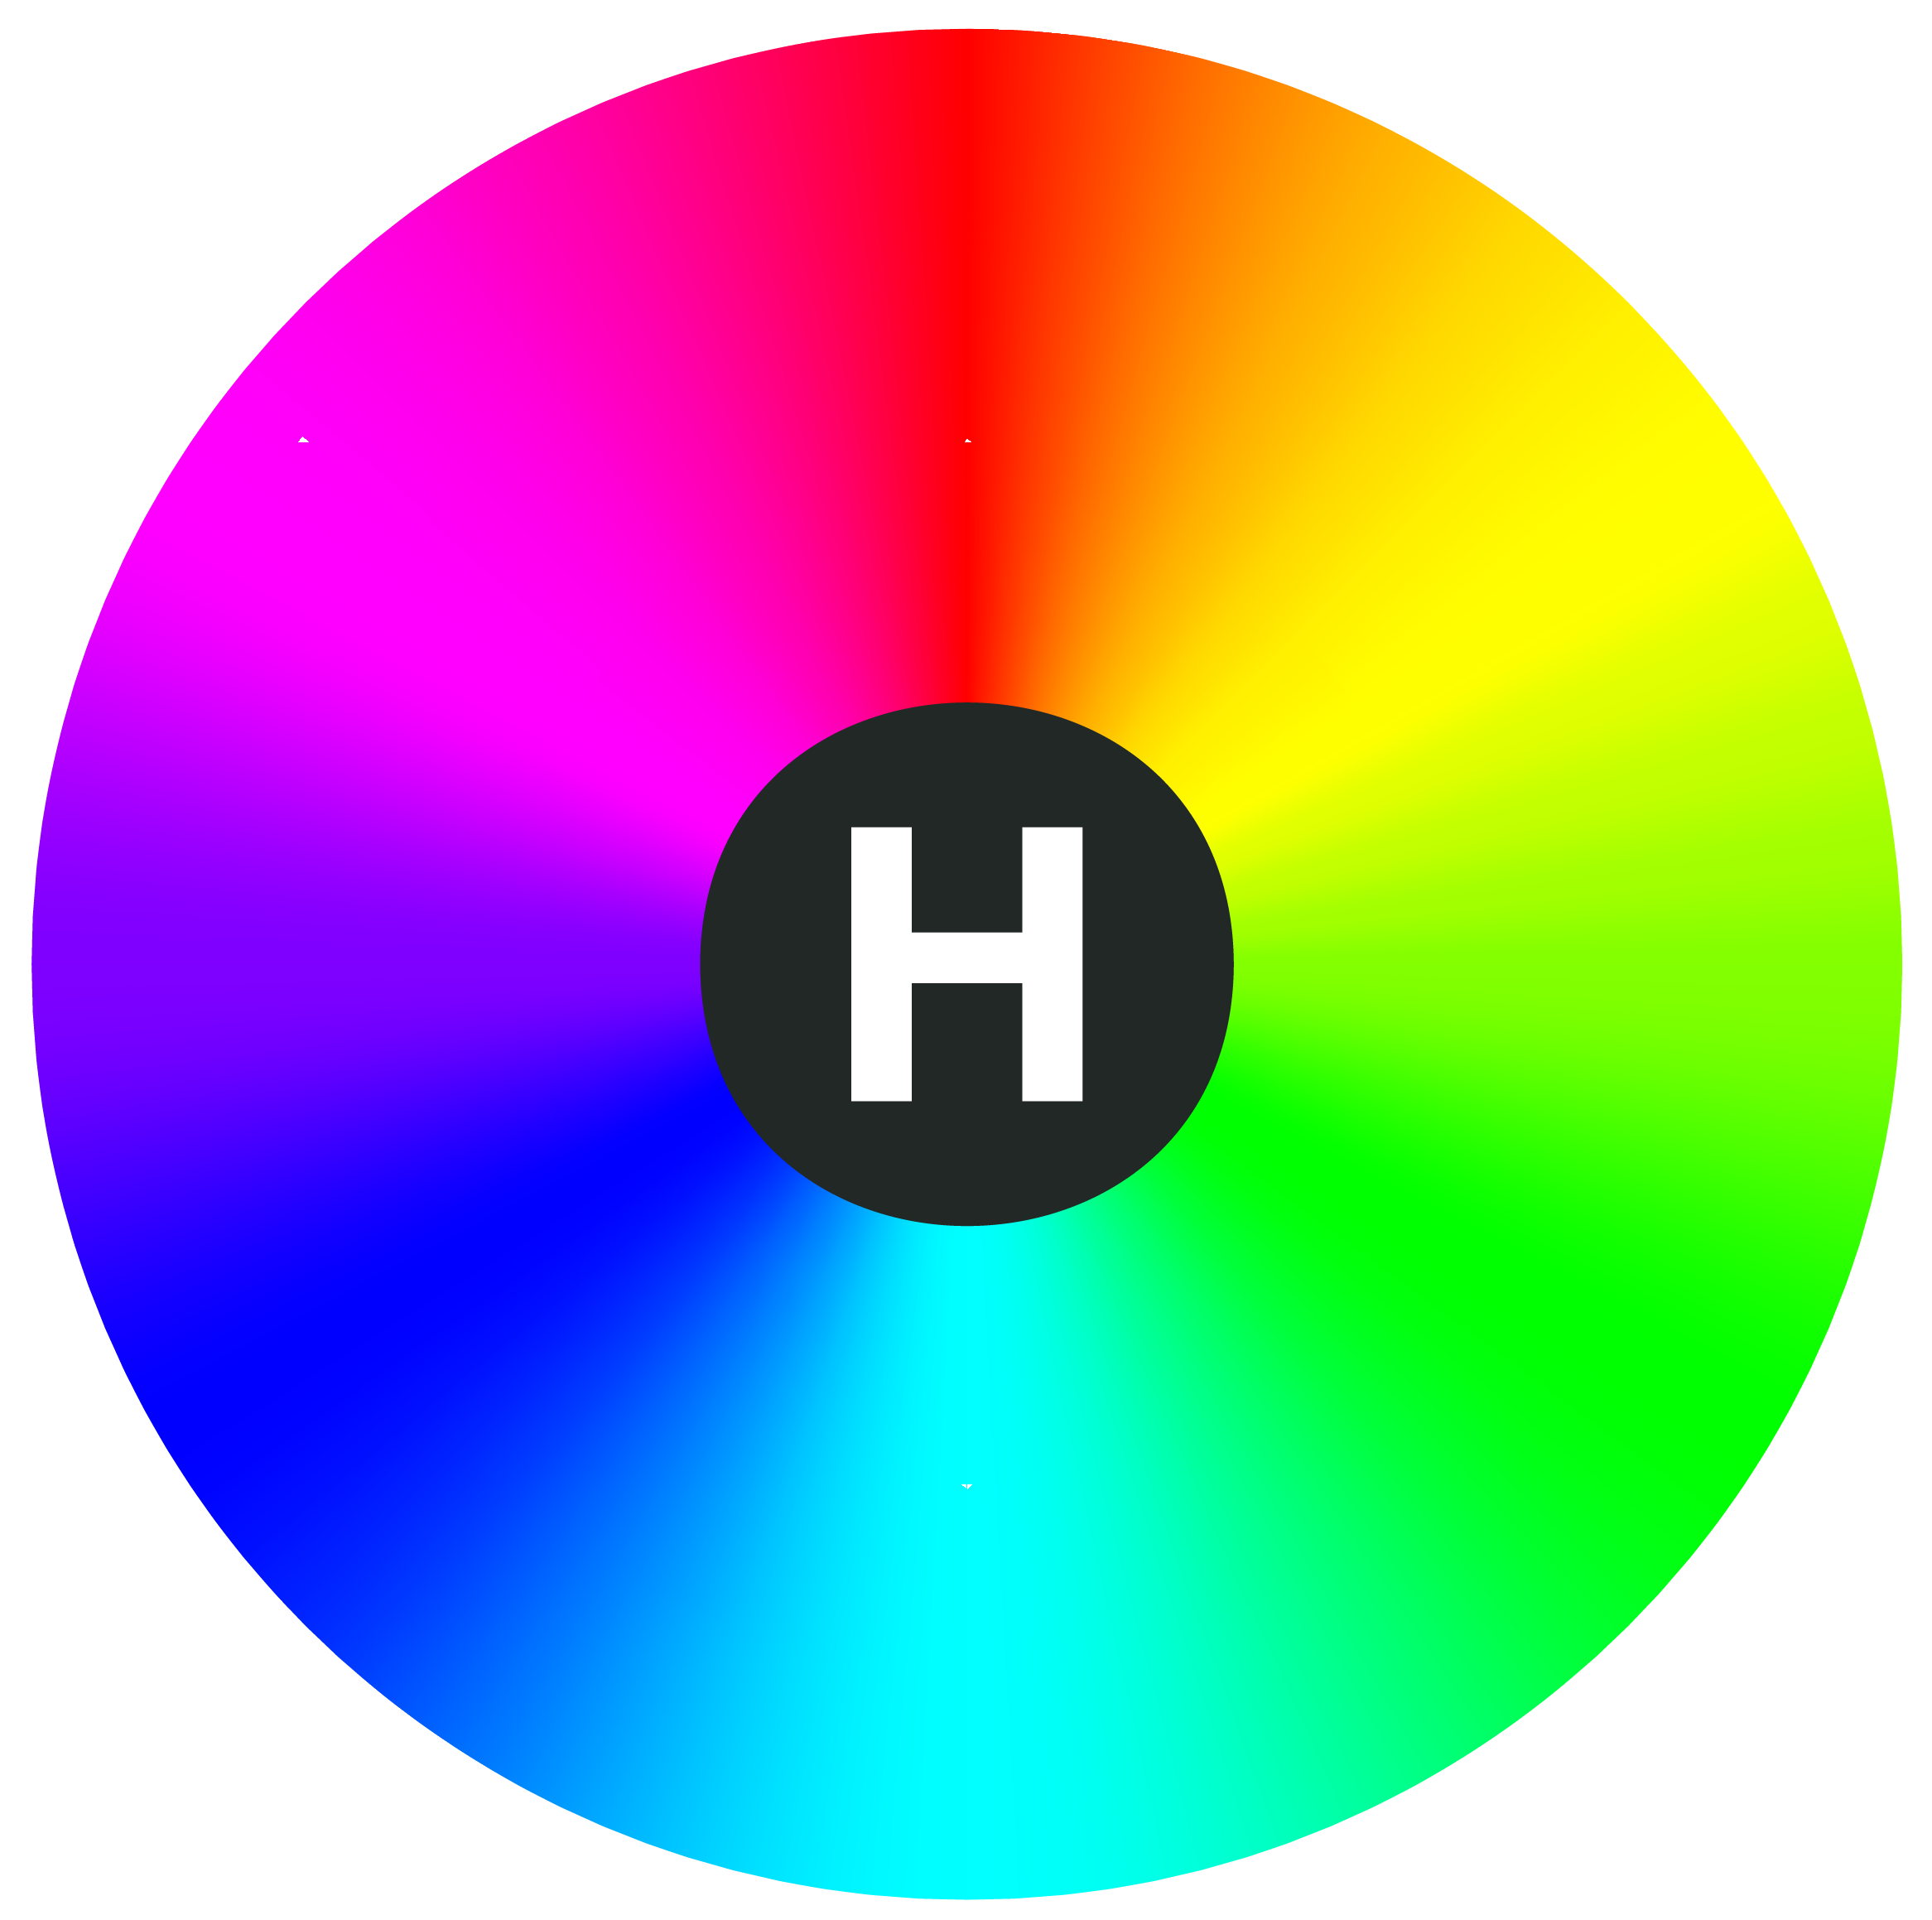
\includegraphics[height=0.7\textwidth]{D6Z/6-7b}
    \end{subfigure}
    \caption{HSL color space – hue}
\end{figure}

Figure 6.8 shows saturation in the HSL color space, ranging from 0\% to 100\%. It describes the changes of color purity under the same hue and lightness. The larger the saturation, the brighter and less gray of the color.

\begin{figure}[h!]
    \centering
    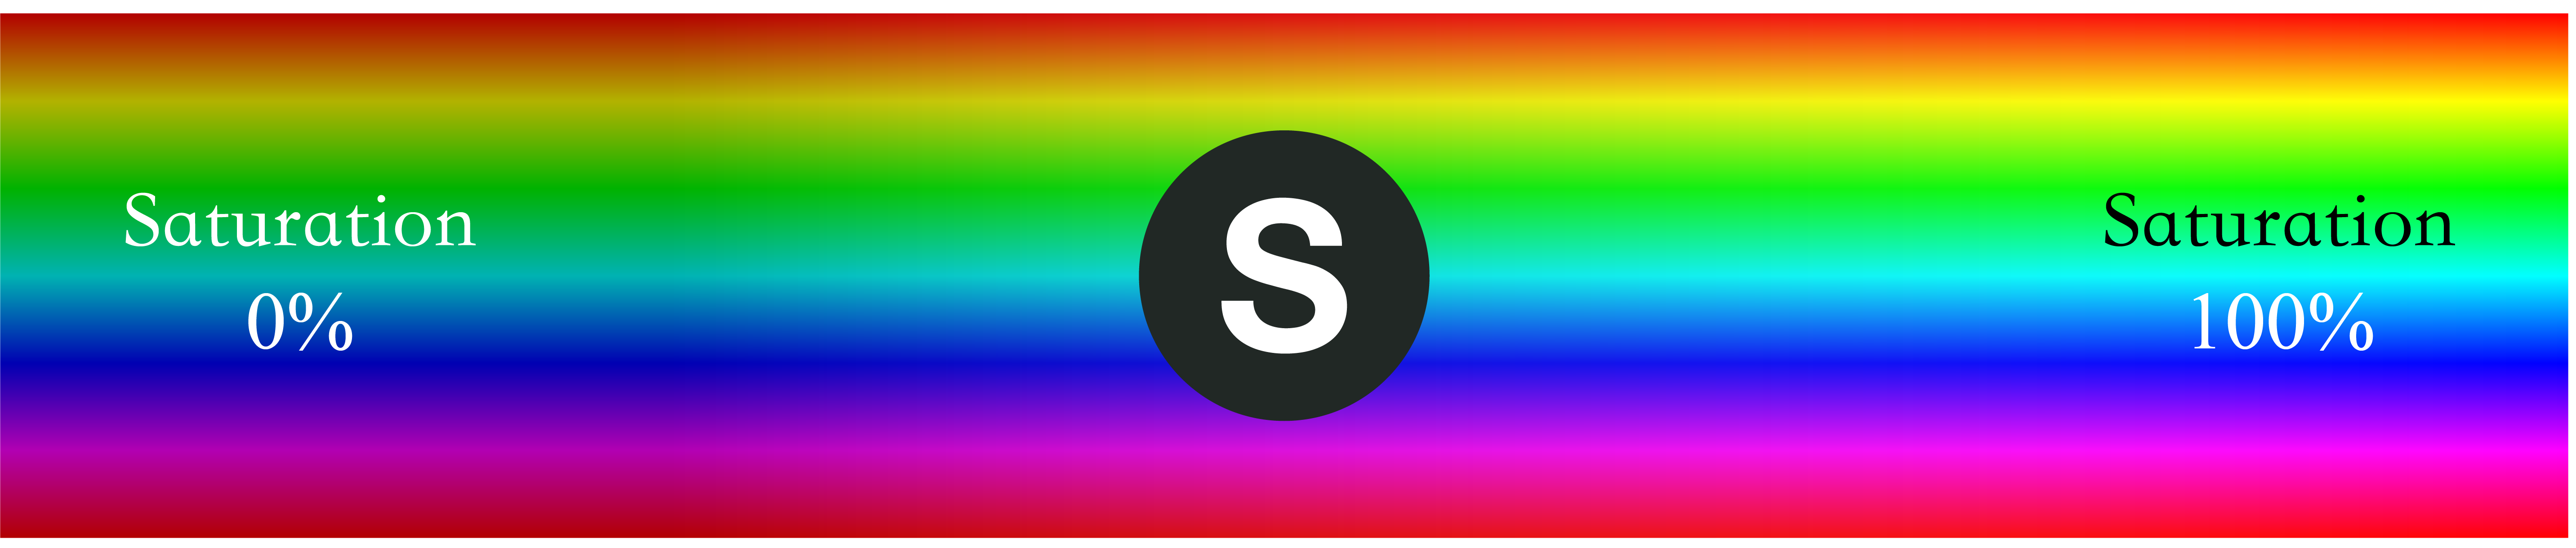
\includegraphics[width=0.6\textwidth]{D6Z/6-8}
    \caption{HSL color space – saturation}
\end{figure}

Figure 6.9 shows lightness in the HSL color space, which represents the luminance of a color. It ranges from 0\% to 100\%. The smaller the value, the darker the color, and the closer to black, and vice versa.

\begin{figure}[h!]
    \centering
    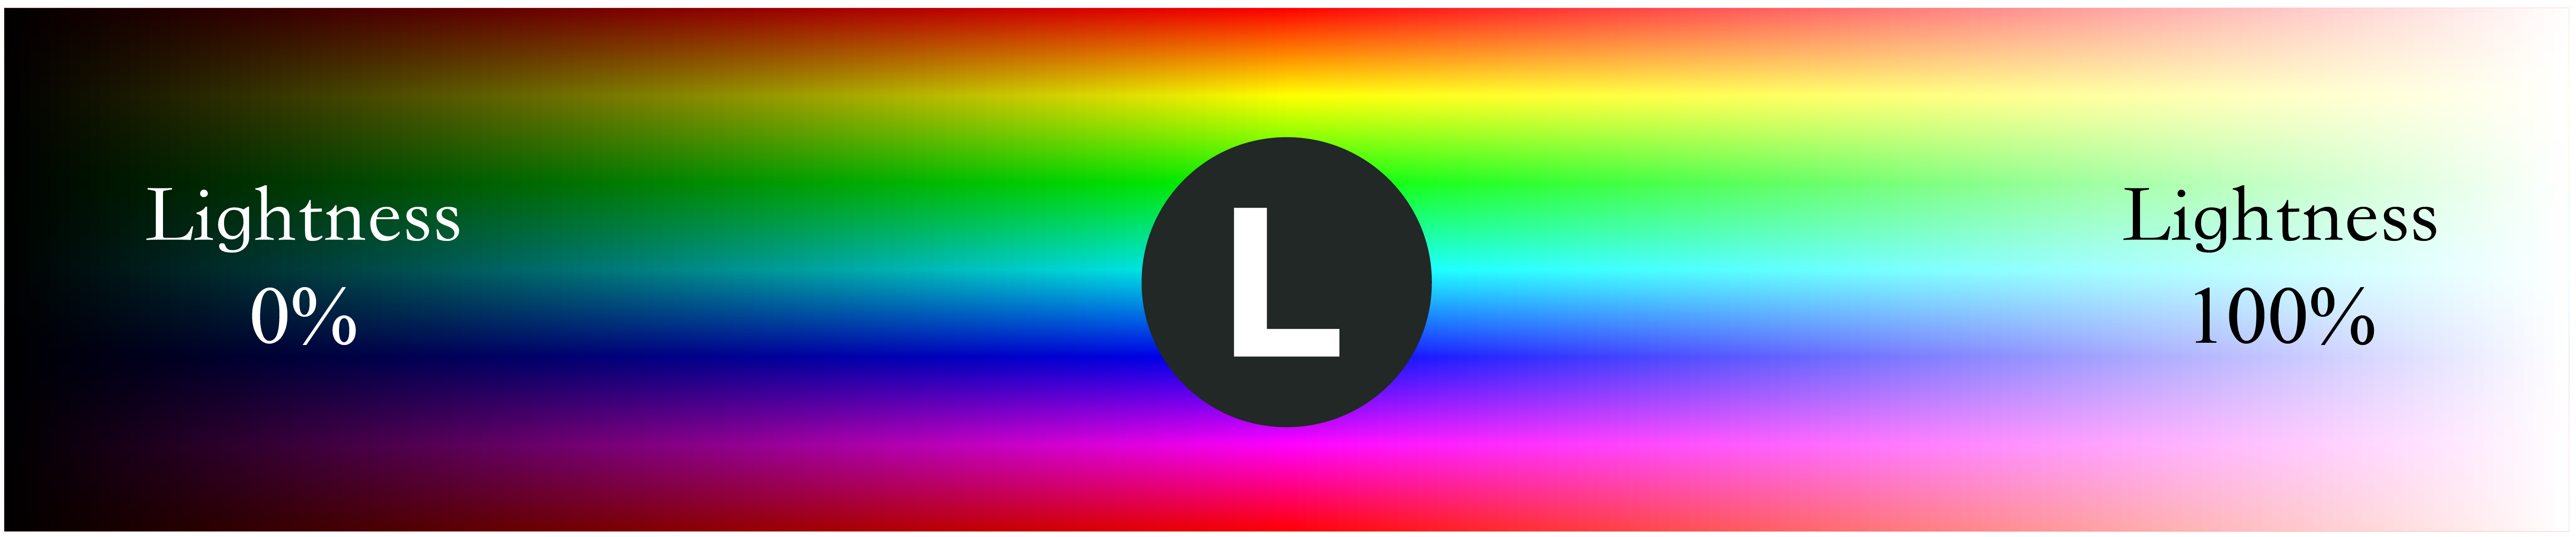
\includegraphics[width=0.6\textwidth]{D6Z/6-9}
    \caption{HSL color space – lightness}
\end{figure}

The three color spaces introduced above merely describe colors from different dimensions, and thus can be mutually converted. In practice, the LED lights uses RGB color space as the brightness of red, green, and blue beads are adjusted to generate various colors. However, the user interface and control commands usually use the HSV or HSL color space. Therefore, the LED driver needs to convert values from the HSV or HSL dimension to the RGB dimension, so as to get the expected LED color.

\subsection{LED Driver}
Compared with traditional light sources, LED is more energy-efficient and eco-friendly with longer lifespan. It is a low-voltage, high-current semiconductor component. Its luminous intensity is positively associated with the forward current. When selecting an LED driver, we need to consider the working environment. If the driver is sensitive to the ambient temperature, we should use components that generate less heat, or dissipate heat. LED driver is a core component of smart lights and will directly affect the lifespan and use experience of smart lights. At present, there are mainly two types of LED drivers.

\begin{term}{Constant-voltage drivers}
    Constant-voltage drivers provide stable terminal voltage for the LED, and the current changes with the load. When driven by a constant-voltage driver, each LED bead needs a suitable resistor to emit light of the same brightness.
\end{term}

\begin{term}{Constant-current drivers}
    Constant-current drivers stablize the current flowing through the LED, and the voltage across the LED changes with the load. When driven by a constant-current driver, the LED can be dimmed by controlling the current flowing through it.
\end{term}

\subsection{LED Dimming}
Dimming is a basic feature of smart LED lights including changing the color, brightness, and on/off status. Users can adjust LED lights through a smartphone app, a remote controller, etc. There are three LED dimming methods.

\begin{term}{TRIAC dimming}
    When using TRIAC dimming, the waveform of the input voltage changes with the conduction angle of the TRIAC, thereby changing the effective value of the input voltage and eventually dimming the LED light. TRIAC dimming is suitable for traditional lamps such as incandescent lamps and fluorescent lamps.
\end{term}

\begin{term}{PWM dimming}
    Basically, PWM switches on/off LED lights and dims lights by sending PWM signals and changing their frequency and duty cycle.
\end{term}

\begin{term}{I2C dimming}
    The constant-current LED linear controller ICs with I2C interfaces are suitable for driving low-power LED lights. Such ICs receive control signals through I2C input interfaces and adjust the current of multiple independent output interfaces to dim the LED.
\end{term}

Among the three LED dimming methods above, PWM dimming performs the best. It guarantees no color shifts and stability at low brightness and is therefore widely used.

Figure 6.10 is the block diagram of PWM dimming, which mainly includes on/off signal sampling circuit, the main control circuit and the PWM controller. The on/off signal sampling circuit generates a clock signal after detecting the on/off signal in the circuit. The main control circuit receives the clock signal and generates three pulse signals, which are respectively output to three PWM controllers. The PWM controllers output different current signals based on the pulse signals to adjust the brightness of corresponding LED bead. The main control circuit usually includes a microcontroller unit, whose input is connected to the on/off signal sampling circuit, and three outputs are respectively connected to three PWM controllers. The outputs of PWM controllers are connected to the red, green, and blue LED beads respectively, thereby controlling their brightness to get the expected color. All LED beads are packaged in one lampshade.

\begin{figure}[h!]
    \centering
    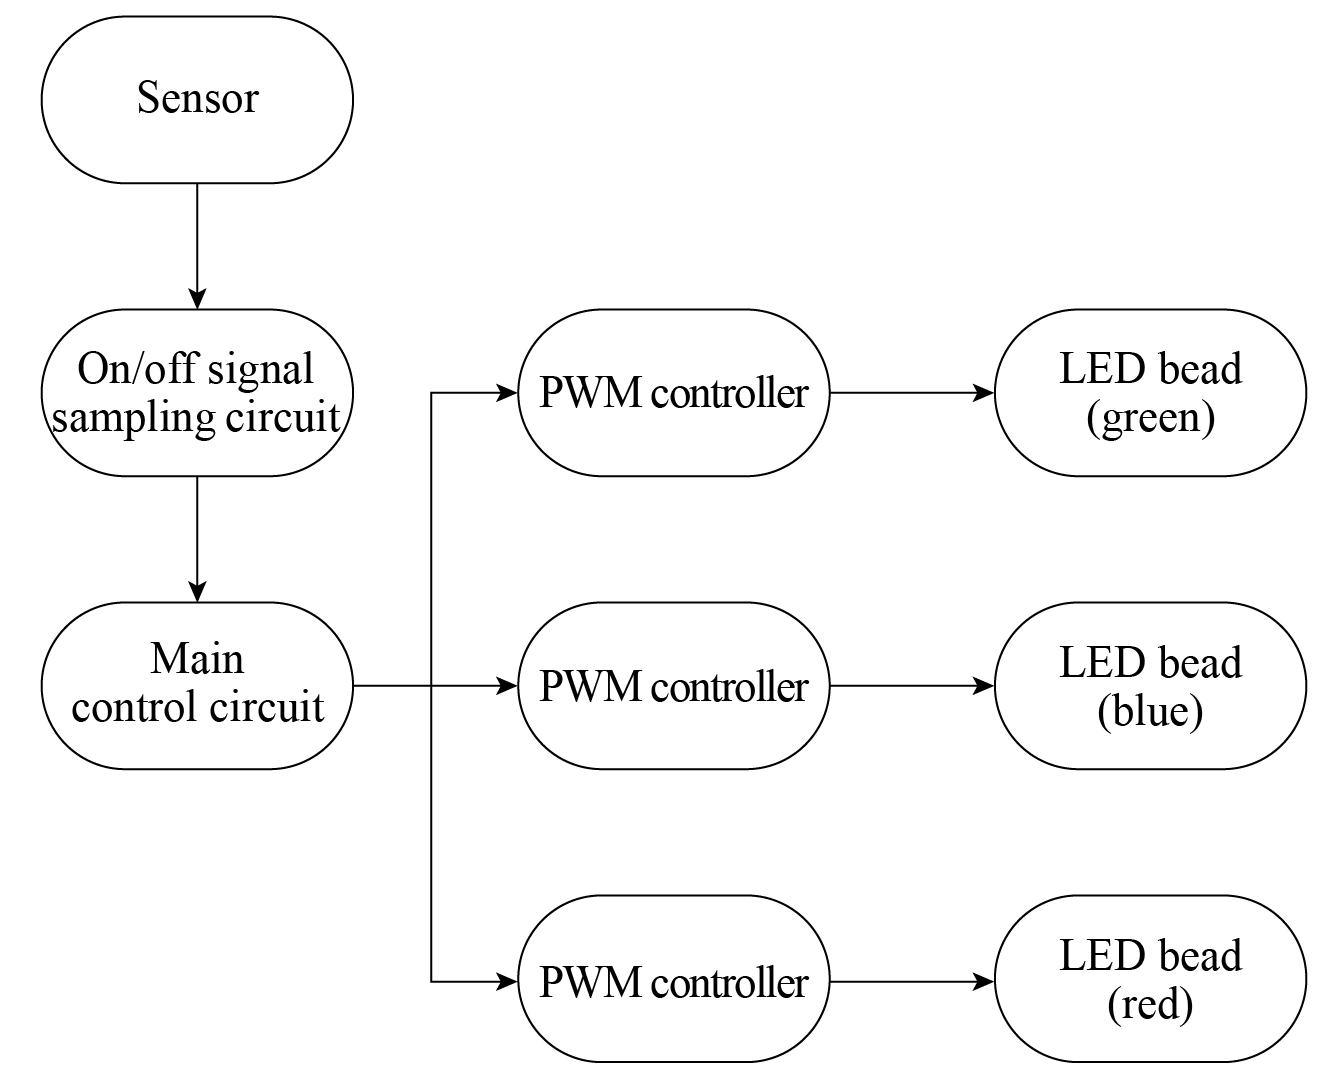
\includegraphics[width=0.6\textwidth]{D6Z/6-10}
    \caption{Block diagram of PWM dimming}
\end{figure}

\subsection{Introduction to PWM}
Pulse width modulation (PWM) is a technique that converts analogue signals into pulse signals (a means of controlling analogue output with digital signals). It can be used to control the brightness of LEDs, the speed of DC motors, etc.

It has three main parameters: frequency, period, and duty cycle. PWM frequency is the number of times the PWM signal goes from high level to low level and back to high level within one second. It is measured in Hz. PWM period is the reciprocal of PWM frequency. PWM duty cycle refers to the ratio of the high-level time to one PWM period, ranging from 0\% to 100\%. Figure 6.11 shows the PWM duty cycle.

\begin{figure}[h!]
    \centering
    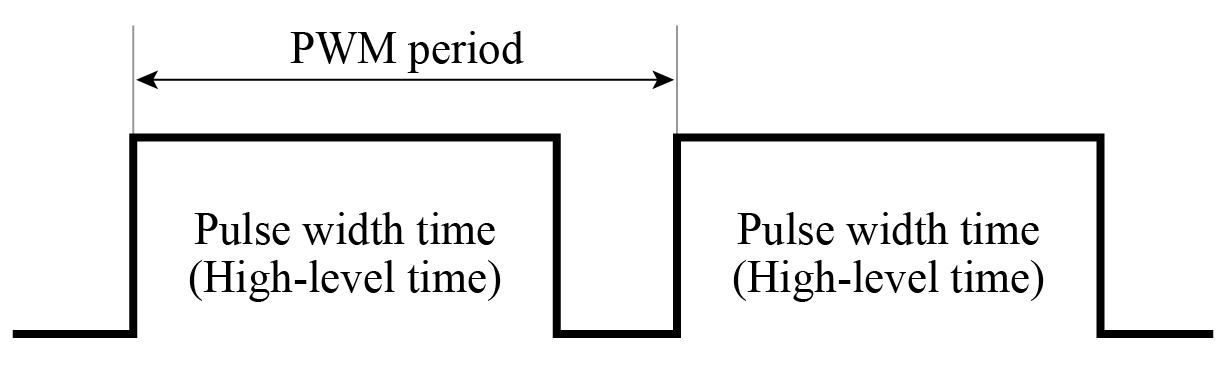
\includegraphics[width=0.6\textwidth]{D6Z/6-11}
    \caption{PWM duty cycle}
\end{figure}

For example, if the PWM period is 10 ms and the pulse width time is 8 ms, then the PWM duty cycle is 8/10=80\%.
    
When using PWM to control an LED, if the light is turned on for 1 second and then off for 1 second repeatedly (i.e., period = 2s, duty cycle = 50\%), the LED will appear to blink. If this cycle is shortened to 200 ms, with the LED being on for 100 ms and then off for 100 ms, the LED will appear to blink at a higher frequency. Due to the persistence of vision, as the cycle continues decreasing, there will be a critical threshold where the human eye cannot perceive the blinking of the LED. At this point, the persistence of vision blends the on and off images, resulting in a stable average brightness. This average brightness is directly related to the PWM duty cycle, as shown in Figure 6.12. Therefore, we can dim LED lights by adjusting the PWM duty cycle.

\begin{figure}[h!]
    \centering
    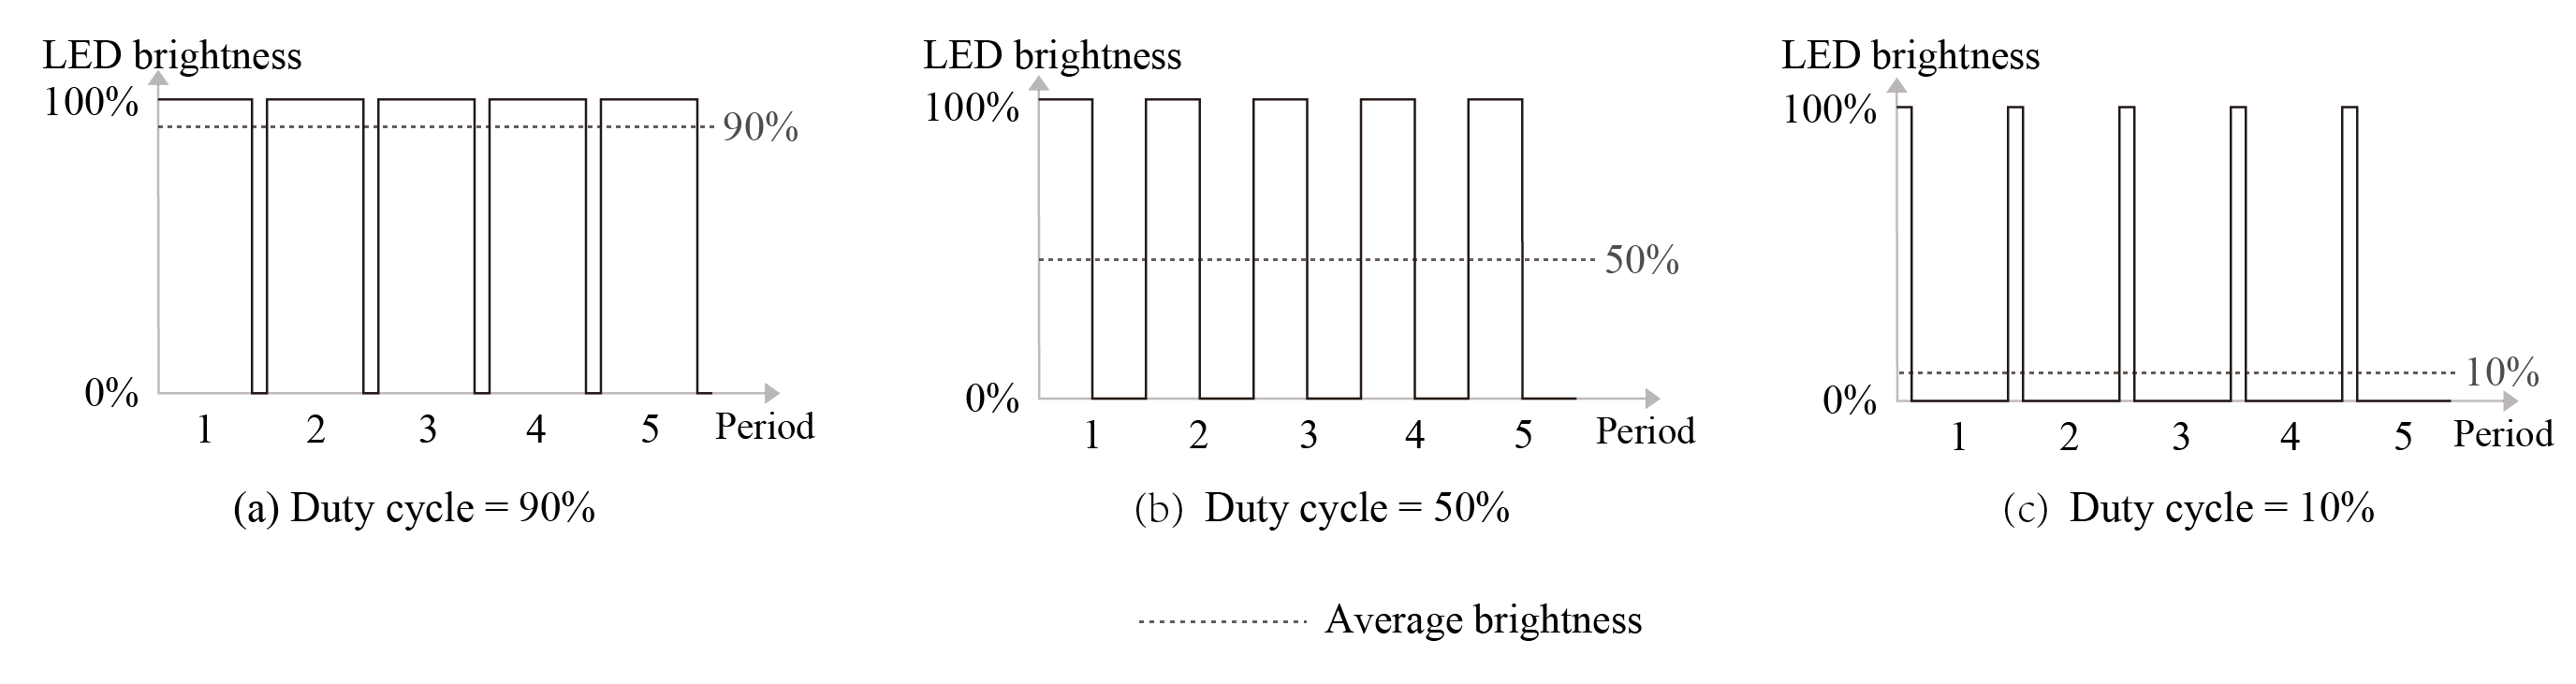
\includegraphics[width=\textwidth]{D6Z/6-12}
    \caption{Relationship between PWM duty cycle and average brightness}
\end{figure}

\section{LED Dimming Driver Development}
After understanding the basics of LED drivers, we can start developing a dimming driver based on the ESP32-C3 chip. This mainly includes the development of functional APIs for controlling the switch, brightness, color, and color temperature. In daily life, it is usually expected to maintain the color, brightness, and color temperature of a light consistent with its previous status when turning it on. This requires preserving the light’s status when it is turned off. To achieve this, we can use the non-volatile storage (NVS) feature provided by ESP-IDF.

So before writing the driver code, it is also necessary to learn about the LED PWM controller of ESP32-C3, its programming procedures, and non-volatile storage.

\subsection{Non-Volatile Storage (NVS)}
The non-volatile storage in ESP-IDF uses a portion of the main flash memory through \verb|esp_|\\ \verb|partition.h| APIs to store key-value pairs. Since NVS is permanent, even if the device is restarted or powered off, the stored data will not be lost. NVS has been specially designed to prevent data corruption caused by power failure, and to distribute the written data throughout NVS in case of flash wear and tear. The dedicated partition in flash used by NVS stores data of various types, such as integers, \verb|NULL|-terminated strings, and binary data.

NVS is suitable for storing small data, rather than large data such as strings or binary large objects (BLOBs) which should be handled by the FAT file system based on wear leveling. In IoT projects, NVS can store not only the unique mass production data for products, but also any user data related to the application.

Following are several key concepts of NVS: key-value pairs, namespaces, security, tamper resistance, and robustness.

\begin{term}{Key-value pairs}
    NVS operates on key-value pairs, as in “key:value”. Keys are ASCII strings of up to 15 characters, while values can be any of the following types:

    \vspace{6pt}
    \begin{itemize}
        \item Integers: \verb|uint8_t|, \verb|int8_t|, \verb|uint16_t|, \verb|int16_t|, \verb|uint32_t|, \verb|int32_t|,\\ \verb|uint64_t|, and \verb|int64_t|.
        \item Strings ending with “0”.
        \item Variable-length binary data.
    \end{itemize}
\end{term}

\begin{term}{Namespaces}
    To mitigate potential conflicts in key names between different components, NVS assigns a namespace to each key-value pair, which follows the same naming rule as keys, i.e., the maximum length is 15 characters. These names are specified in the \verb|nvs_open()| or \verb|nvs_open_from_part()| call. This call returns an opaque handle, which is used in subsequent calls to \verb|nvs_get_*()|, \verb|nvs_set_*()|, and \verb|nvs_commit()| functions. In this way, a handle is associated with each namespace, and key names will not collide with the same names in other namespaces. Please note that the namespaces with the same name in different NVS partitions are considered as separate namespaces.
\end{term}

\begin{term}{Security, tamper resistance, and robustness}
    After NVS encryption, data will be stored in encrypted form. If NVS encryption is not enabled, any user with physical access to the flash can modify, erase, or add key-value pairs. If NVS encryption is enabled, key-value pairs cannot be modified or added without knowing the corresponding NVS encryption key. However, there is no tamper-resistance against the erase operation.

    \vspace{6pt}
    When the flash runs into an inconsistent state, NVS will try recovering. Powering off a device at any time and then powering it back on will not cause data loss. However, if the device is powered off while writing a new key-value pair, that specific pair may be lost.
\end{term}

\subsection{LED PWM Controller (LEDC)}
The LED PWM controller of ESP32-C3 can generate six independent digital waveforms, with the following features:

\begin{itemize}[noitemsep]
    \item Six independent PWM generators (i.e., six channels)
    \item Four independent timers that support division by fractions
    \item Automatic duty cycle fading (i.e., gradual increase/decrease of a PWM’s duty cycle without interference from ESP32-C3) with interrupt generation on fade completion
    \item Adjustable phase of PWM signal output
    \item PWM signal in Light-sleep mode (see details of low-power modes in Chapter 12)
    \item Maximum PWM resolution: 14 bits
\end{itemize}

The four timers are identical regarding their features and operation. The following sections refer to the timers collectively as Timer\textit{x} (where \textit{x} ranges from 0 to 3). Likewise, the six PWM generators are also identical in features and operation, and thus are collectively referred to as PWM\textit{n} (where \textit{n} ranges from 0 to 5). Figure 6.13 shows the LED PWM timer.

\begin{figure}[h!]
    \centering
    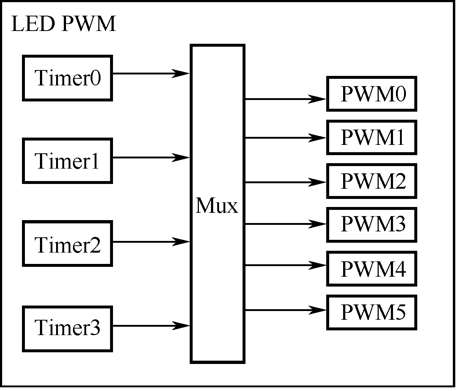
\includegraphics[width=0.5\textwidth]{D6Z/6-13}
    \caption{LED PWM timer}
\end{figure}

The four timers can be independently configured (i.e., configurable clock divider, and counter overflow value) and each internally maintains a timebase counter (i.e., a counter that counts on cycles of a reference clock). Each PWM generator selects one of the four timers, uses the timer’s counter value as a reference to generate PWM signals, and outputs the signals to the timer.

Figure 6.14 shows the main functional blocks of the timer and the PWM generator.

    \begin{figure}[h!]
    \centering
    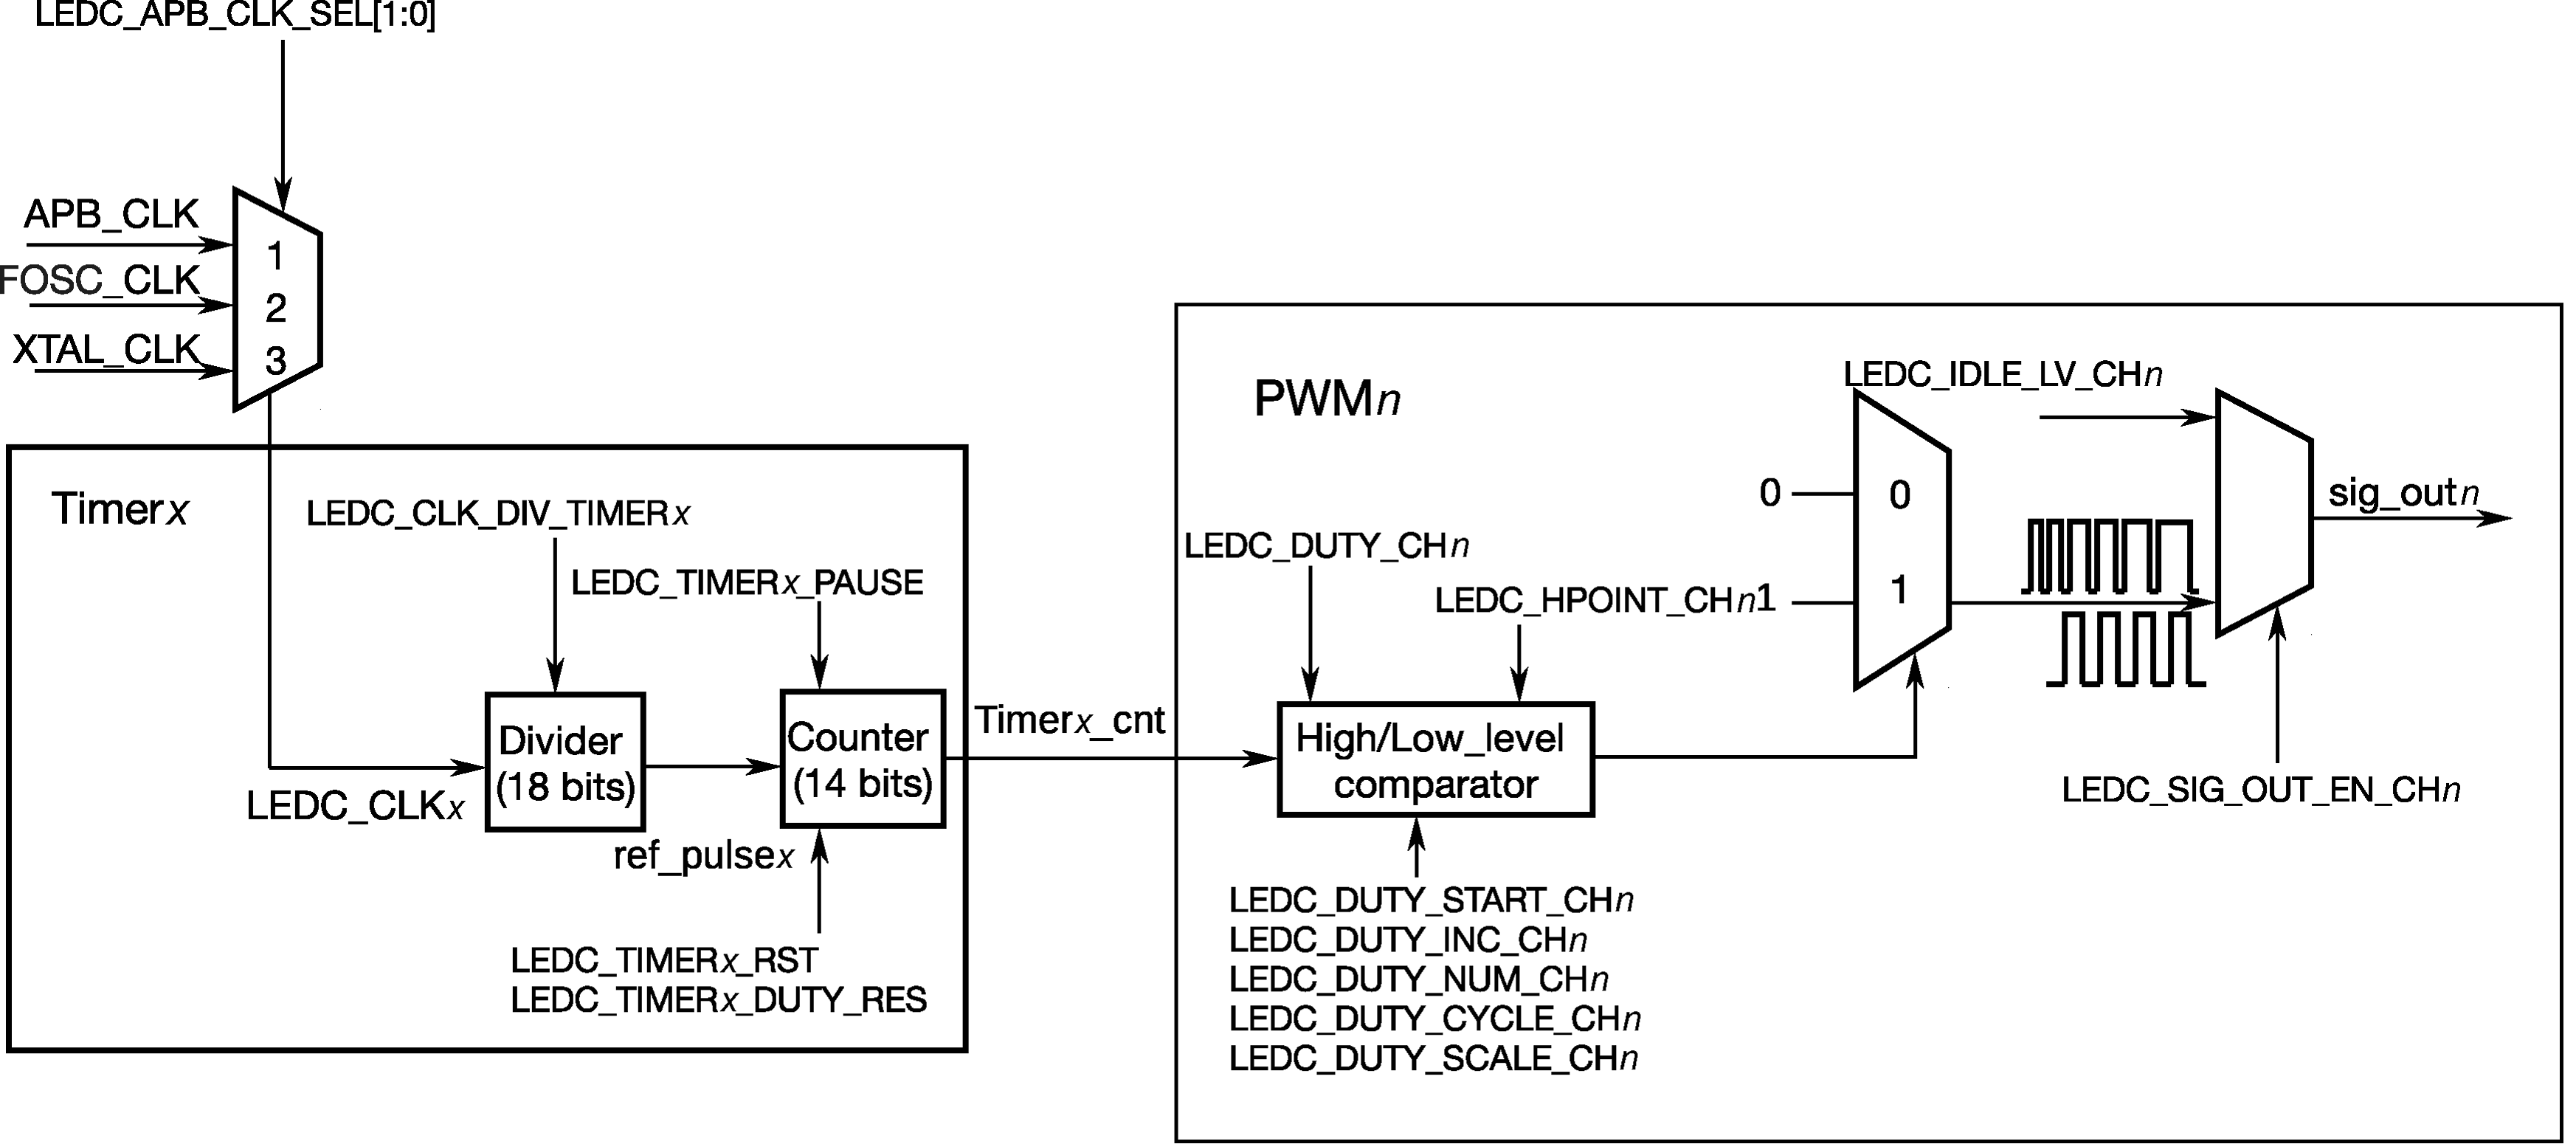
\includegraphics[width=\textwidth]{D6Z/6-14}
    \caption{Functional blocks of LED PWM timer and generator}
    \end{figure}

To generate PWM signals, a PWM generator (PWM\textit{n}) needs to select one of the four timers (Timer\textit{x}) and use its counter value as a reference to generate signals. Each PWM generator has a comparator and two multiplexers. It compares the timer’s 14-bit counter value (timer\textit{x}\_cnt) to two trigger values of the comparator hpoint\textit{n} and lpoint\textit{n}. When timer\textit{x}\_cnt equals hpoint\textit{n} or lpoint\textit{n}, high- or low-level PWM signal will be generated respectively.

Figure 6.15 shows how hpoint\textit{n} and lpoint\textit{n} are used to generate PWM signals with a fixed duty cycle.

\begin{figure}[h!]
    \centering
    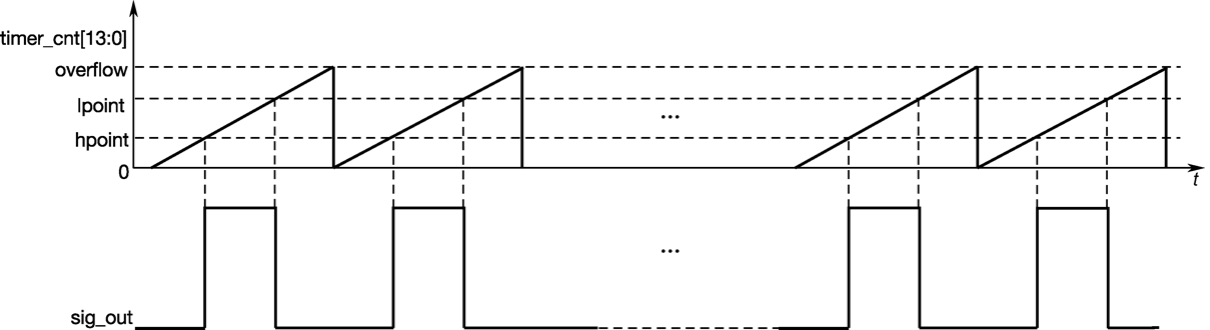
\includegraphics[width=\textwidth]{D6Z/6-15}
    \caption{Generating PWM signals with a fixed duty cycle using hpoint\textit{n} and lpoint\textit{n}}
\end{figure}

PWM generators can fade the duty cycle of a PWM output signal. When duty cycle fading is enabled, the value of lpoint\textit{n} will be incremented/decremented every time the counter overflows a certain number of times. Figure 6.16 demonstrates the process of duty cycle fading.

\begin{figure}[h!]
    \centering
    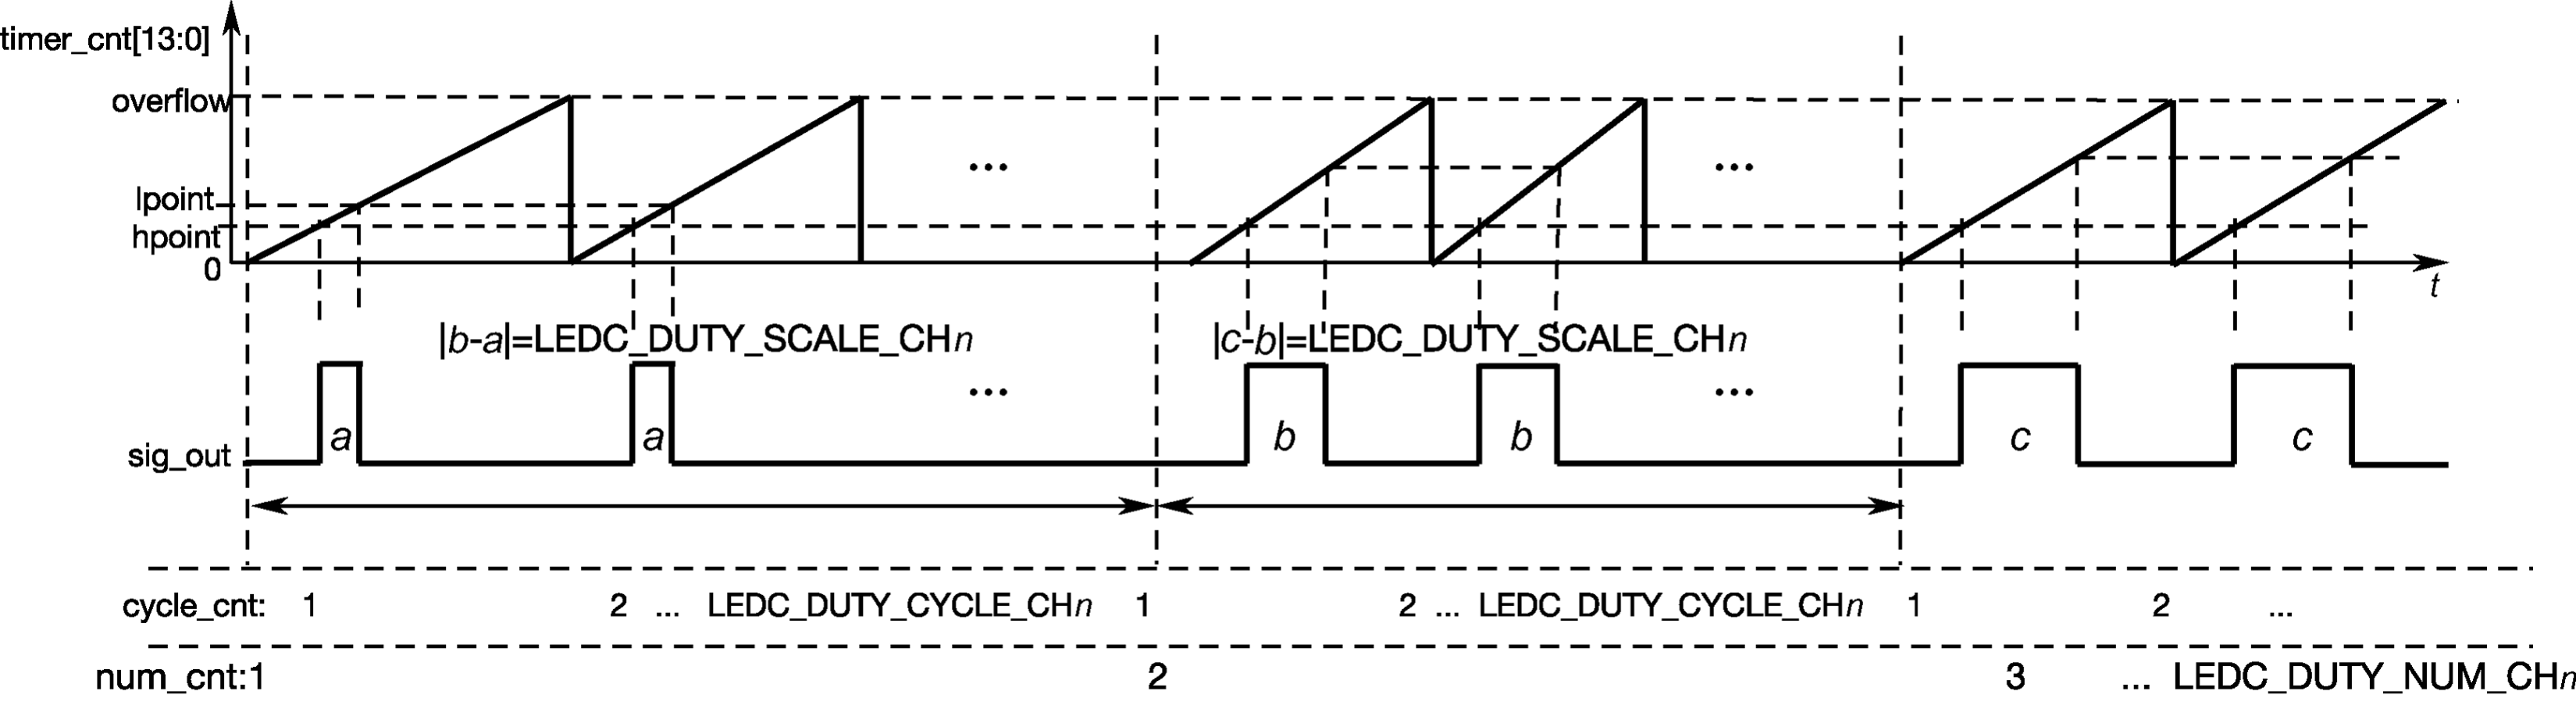
\includegraphics[width=\textwidth]{D6Z/6-16}
    \caption{Duty cycle fading}
\end{figure}

\subsection{LED PWM Programming}
Having learned about the LEDC of ESP32-C3, now we need to configure the controller using LED PWM APIs provided by ESP-IDF. The configuration includes three steps, as shown in Figure 6.17.

\begin{enumerate}[label=\arabic*.,noitemsep]
    \item \textbf{Configure the timer}, specifying the frequency and duty resolution of PWM signals.
    \item \textbf{Configure the channel}, mapping the timer to the GPIOs that output PWM signals.
    \item \textbf{Output PWM signals} to drive the LED. The brightness of the LED can be changed through software control or the hardware’s duty cycle fading function.
\end{enumerate}

\begin{figure}[h!]
    \centering
    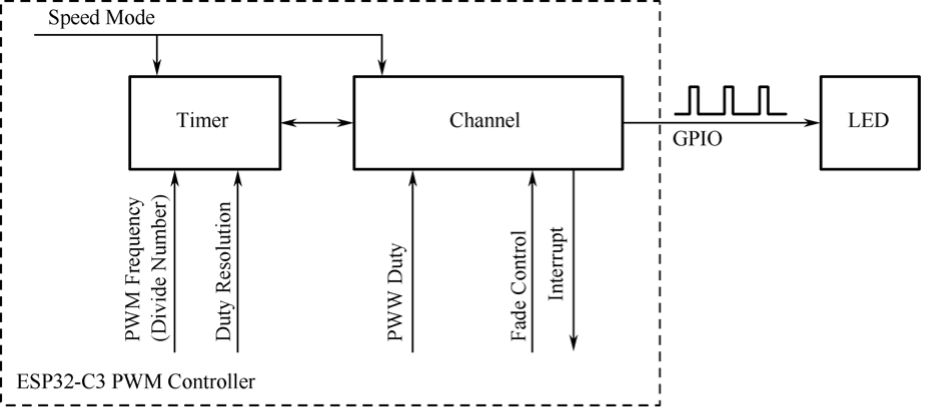
\includegraphics[width=0.7\textwidth]{D6Z/6-17}
    \caption{Steps of configuring PWM controller}
\end{figure}

\subsubsection{1. Configuring the timer}
Timers can be configured by calling \verb|ledc_timer_config()|, when an \verb|ledc_timer_|\\ \verb|config_t| structure with the following parameters needs to be passed to the function:

\begin{itemize}[noitemsep]
    \item Speed mode (the value of this parameter must be \verb|LEDC_LOW_SPEED_MODE|);
    \item Timer index \verb|timer_num|;
    \item PWM frequency;
    \item PWM duty resolution.
\end{itemize}

PWM frequency is inversely proportional to duty resolution, as higher frequency results in fewer available duty cycles for a given period and vice versa. This interrelationship may be more important if the API is used for purposes other than changing the brightness of LEDs.

\subsubsection{2. Configuring the channel}
After configuring the timer, you also need to configure the required channel (one of \verb|ledc_|\\ \verb|channel_t|) by calling \verb|ledc_channel_config()|. An \verb|ledc_channel_config_t| structure with channel configuration parameters needs to be passed to the function.

Then the channel will start operating according to the \verb|ledc_channel_config_t| structure and generate PWM signals on the selected GPIOs with the frequency specified in step 1 and the duty cycle specified in step 2. This process can be suspended at any time by calling the \verb|ledc_stop()| function.

\subsubsection{3. Changing PWM signals}
Once the channel starts operating and generating the PWM signal with a constant duty cycle and frequency, there are a couple of ways to change this signal. For LED dimming, we primarily change the duty cycle to vary the light color and brightness.

\begin{term}{Changing PWM duty cycle using software}
    To set the duty cycle, use the dedicated function \verb|ledc_set_duty()|. After that, call \verb|ledc_update_duty()| to activate the changes. To check the currently set value, use the function \verb|ledc_get_duty()|.

    \parskip 6pt
    Another way to set the duty cycle, as well as some other channel parameters, is by calling \verb|ledc_channel_config()|.

    The PWM duty cycle passed to the function depends on \verb|duty_resolution|, and the value ranges from 0 to 2$^{\verb|duty_resolution|}$--1. For example, if \verb|duty_resolution| is 10, then the duty cycle values can range from 0 to 1023.
\end{term}

\begin{term}{Changing PWM duty cycle using hardware}
    LEDCs provide the means to gradually change (fade) the duty cycle. To use this functionality, enable fading with \verb|ledc_fade_func_install()| and then configure it by calling one of the following functions.

\parskip 6pt
\begin{codebloc}
\begin{tabular}{a}
\vspace{2pt}
\begin{verbatim}
1.  esp_err_t ledc_set_fade_with_time(ledc_mode_t speed_mode,
2.                                  ledc_channel_t channel,
3.                                  uint32_t target_duty,
4.                                  int max_fade_time_ms);
5.	
6.  esp_err_t ledc_set_fade_with_step(ledc_mode_t speed_mode,
\end{verbatim}
\verb|7.                                  ledc_channel_t channel,|
\end{tabular}
\end{codebloc}

\begin{codebloc}
\begin{tabular}{a}
\vspace{2pt}
\begin{verbatim}
8.                                  uint32_t target_duty,
9.                                  uint32_t scale,
10.                                 uint32_t cycle_num);
11.	
12. esp_err_t ledc_set_fade(ledc_mode_t speed_mode,
13.                         ledc_channel_t channel,
14.                         uint32_t duty,
15.                         ledc_duty_direction_t fade_direction,
16.                         uint32_t step_num,
17.                         uint32_t duty_cycle_num,
\end{verbatim}
\verb|18.                         uint32_t duty_scale);|
\end{tabular}
\end{codebloc}

    Finally, call \verb|ledc_fade_start()| to initiate fading. If not required anymore, the fading can be disabled with \verb|ledc_fade_func_uninstall()|.
\end{term}

\subsubsection{4. Range of PWM frequency and duty resolution}
The LED PWM controller is mainly used for driving LED dimming. It provides a large flexibility of PWM duty cycle settings. For instance, the PWM frequency of 5 kHz can have the maximum duty resolution of 13 bits. This means that the duty can be set anywhere from 0\% to 100\% with a resolution of $\sim$0.012\% (2$^{13}$ = 8192 discrete levels of LED brightness). Please note that these parameters depend on the clock signal clocking the LED PWM controller timer which in turn clocks the channel.

The LEDC can be used for generating signals with higher frequencies that are sufficient to clock other devices such as digital camera modules. In this case, the maximum frequency can be 40 MHz with duty resolution of 1 bit. This means that the duty cycle is fixed at 50\% and cannot be adjusted.

The LEDC API will report an error when the configured frequency and duty resolution exceed the range of LEDC’s hardware. For example, an attempt to set the frequency to 20 MHz and the duty resolution to 3 bits will result in the following error reported on a serial monitor:

\begin{codebloc}
\begin{tabular}{d}
\verb|[E (196) ledc: requested frequency and duty resolution cannot be achieved, try |

\verb|reducing freq_hz or duty_resolution. div_param=128]|
\end{tabular}  
\end{codebloc}

In such a situation, either the duty resolution or the frequency must be reduced. For example, setting the duty resolution to 2 bits can solve this problem and will make it possible to set the duty cycle at 25\% steps, i.e., at 25\%, 50\%, or 75\%.

The LEDC driver will also capture and report attempts to configure frequency / duty resolution combinations that are below the supported minimum, e.g.:

\begin{codebloc}
\begin{tabular}{d}
\verb|[[E (196) ledc: requested frequency and duty resolution cannot be achieved, try |

\verb|increasing freq_hz or duty_resolution. div_param=128000000]]|
\end{tabular}  
\end{codebloc}

The duty resolution is normally set by \verb|ledc_timer_bit_t|, with a range of 10 to 15 bits. For smaller duty resolutions (from 10 down to 1), just enter the equivalent numeric directly.

\section{Practice: Adding Drivers to Smart Light Project}
There are two drivers to be developed in a smart light project – the button driver and the LED dimming driver. With these two drivers, we can use a button to control LEDs.

\subsection{Button Driver}
When using ESP32-C3-DevKitM-1 to simulate smart light for development, we can find two buttons on the board, namely the Boot button and the RST button. The RST button is used for resetting and restarting ESP32-C3, while the Boot button functions as a regular button once the firmware starts operating. In other words, the Boot button can be used to simulate a light switch.

For this purpose, we introduce the \verb|button| component as the button driver. You may read the source code to learn about its development, as we will not expound on it in this book. To add the driver to the smart light project, please follow the steps below.

\subsubsection{1. Adding driver-related source files}
Create a folder named \verb|components| under the directory of the smart light project and put the components used by the project into the folder.

Create a subfolder named \verb|button| under \verb|components|.

Then, create the source files and header files for the button driver in \verb|button|, and edit the code accordingly.

Specific code can be found from \href{https://github.com/espressif/book-esp32c3-iot-projects/tree/main/device_firmware/components/button}{\texttt{book-esp32c3-iot-projects/device\_firmware/\\ components/button}}.

In the \verb|main| folder of the project, create a source file named \verb|app_driver.c| to process all the drivers. Meanwhile, create header files in the \verb|include| folder under \verb|main|. Add driver operations and function declarations to corresponding files, such as driver initialization and button event processing. The key code is as follows.

\begin{codebloc}
\begin{tabular}{d}
\vspace{2pt}
\begin{verbatim}
1.  //Callback function for pressing the button
2.  static void push_btn_cb(void *arg)
3.  {
4.      //Code Omitted
5.  }
6.  void app_driver_init()
7.  {
8.      //Initializing button driver
9.      button_config_t btn_cfg = {
10.             .type = BUTTON_TYPE_GPIO,
11.             .gpio_button_config = {
\end{verbatim}
\verb|12.                 .gpio_num     = LIGHT_BUTTON_GPIO,|
\end{tabular}
\end{codebloc}

\begin{codebloc}
\begin{tabular}{d}
\vspace{2pt}
\begin{verbatim}
13.                 .active_level = LIGHT_BUTTON_ACTIVE_LEVEL,
14.             },
15.         };
16.         button_handle_t btn_handle = iot_button_create(&btn_cfg);
17.         if (btn_handle) {
18.           iot_button_register_cb(btn_handle, BUTTON_PRESS_UP, push_btn_cb);
19.         }
20.         //Code Omitted
\end{verbatim}
\verb|21. }|
\end{tabular}
\end{codebloc}

\subsubsection{2. Adding source files to the compiling system}
First, edit the \verb|CMakeLists.txt| file under the \textbf{project directory}. Append the path of the components in \verb|components| to the search path with the following code:

\begin{codebloc}
\begin{tabular}{d}
\vspace{2pt}
\begin{verbatim}
1.  //Code Omitted
2.  set(EXTRA_COMPONENT_DIRS ${CMAKE_CURRENT_LIST_DIR}/../components)	
\end{verbatim}
\verb|3.  //Code Omitted|
\end{tabular}
\end{codebloc}

Then, edit the \verb|CMakeLists.txt| file in the \textbf{\texttt{main} folder}. Add the source file \verb|app_driver.c| to the compiling system with the following code:

\begin{codebloc}
\begin{tabular}{d}
\vspace{2pt}
\begin{verbatim}
1.  set(srcs "app_main.c"
2.           "app_driver.c")
3.  set(include_dirs "include")
4.  idf_component_register(SRCS "${srcs}"
\end{verbatim}
\verb|5.                        INCLUDE_DIRS "${include_dirs}")|
\end{tabular}
\end{codebloc}

Besides, the \verb|button| component also has a \verb|CMakeLists.txt| file, which is used to add the button driver source code to the compiling system. You may refer to \href{https://github.com/espressif/book-esp32c3-iot-projects/blob/main/device_firmware/components/button/CMakeLists.txt}{\texttt{book-esp32c3-iot\\ -projects/device\_firmware/components/button/CMakeLists.txt}} for details. Other components to be added have similar structures and will not be explained again in subsequent chapters.

\subsection{LED Dimming Driver}
The LED lights used in our project have five color options: red, green, blue, warm (WW), and cold (CW), so we need five PWM channels to control them. The target functions include turning on/off LED lights, and controlling their color, color temperature, brightness, breathing, and fading. However, since we are using the ESP32-C3-DevKitM-1 in practice, which only has R, G, and B channels, we can only change LEDs’ colors but not their color temperature during development.

According to the requirements of the smart light project, the LED dimming driver is encapsulated and provided in the form of a \verb|light_driver| component, which can be found at \href{https://github.com/espressif/book-esp32c3-iot-projects/tree/main/device_firmware/components/light_driver}{\texttt{book-esp32c3-iot-projects/device\_firmware/components/light\_driver}}.

Besides, to save the status of LED lights, the project also introduces an \verb|app_storage| component. Its underlayer adopts NVS, which stores key-value pairs in the main flash partition by calling APIs in \verb|esp_partition.h|. The component can be found at \href{https://github.com/espressif/book-esp32c3-iot-projects/tree/main/device_firmware/components/app_storage}{\texttt{book-esp32c3-\\ iot-projects/device\_firmware/components/app\_storage}}.

\subsubsection{1. \texttt{light\_driver} component}
According to the requirements of this project, the \verb|light_driver| component implements functions such as initializing/deinitializing the LED dimming driver, turning on/off lights, controlling their color, brightness, color temperature, etc. Table 6.1 lists the APIs provided for the main application by the LED dimming driver in the \verb|light_driver| component.

{\renewcommand{\arraystretch}{1.2}
\begin{longtable}{|>{\footnotesize}m{0.46\textwidth}|>{\footnotesize}m{0.52\textwidth}|}
    \caption{APIs provided by the LED dimming driver in \texttt{light\_driver}\label{6.1}} \\
        
    \hline
    \rowcolor{LightBlue}\multicolumn{1}{|c|}{\textbf{API}}&\multicolumn{1}{c|}{\textbf{Function}}\\
    \hline
    \endfirsthead

    \multicolumn{2}{r}{Continuation of Table \ref{6.1}}\\
    \hline
    \rowcolor{LightBlue}\multicolumn{1}{|c|}{\textbf{API}}&\multicolumn{1}{c|}{\textbf{Function}}\\
    \hline
    \endhead
        
    \verb|light_driver_init()|&Initialize \verb|light_driver|\\
    \hline
    \verb|light_driver_deinit()|&Deinitialize \verb|light_driver|\\
    \hline
    \verb|light_driver_config()|&Configure fade time and blink cycle of \verb|light_driver|\\
    \hline
    \verb|light_driver_set_switch()|&Turn on/off LED lights\\
    \hline
    \verb|light_driver_get_switch()|&Get the on/off status of LED lights\\
    \hline
    \verb|light_driver_set_hue()|&Set the Hue\\
    \hline
    \verb|light_driver_get_hue()|&Get the Hue\\
    \hline
    \verb|light_driver_set_saturation()|&Set the Saturation\\
    \hline
    \verb|light_driver_get_saturation()|&Get the Saturation\\
    \hline
    \verb|light_driver_set_value()|&Set the Value (as in HSV)\\
    \hline
    \verb|light_driver_get_value()|&Get the Value (as in HSV)\\
    \hline
    \verb|light_driver_set_hsv()|&Set the three HSV components in one call\\
    \hline
    \verb|light_driver_get_hsv()|&Get the three HSV components in one call\\
    \hline
    \verb|light_driver_set_lightness()|&Set the Lightness (as in HSL)\\
    \hline
    \verb|light_driver_get_lightness()|&Get the Lightness (as in HSL)\\
    \hline
    \verb|light_driver_set_hsl()|&Set the three HSL components in one call\\
    \hline
    \verb|light_driver_get_hsl()|&Get the three HSL components in one call\\
    \hline
    \verb|light_driver_set_color_temperature()|&Set the color temperature\\
    \hline
    \verb|light_driver_get_color_temperature()|&Get the color temperature\\
    \hline
    \verb|light_driver_set_brightness()|&Set the brightness\\
    \hline
    \verb|light_driver_get_brightness()|&Get the brightness\\
    \hline
    \verb|light_driver_set_ctb()|&Set color temperature and brightness in one call\\
    \hline
    \verb|light_driver_get_ctb()|&Get color temperature and brightness in one call\\
    \hline
    \verb|light_driver_set_rgb()|&Set the three RGB components in one call\\
    \hline
    \verb|light_driver_breath_start()|&Set the color of LED breathing and start breathing\\
    \hline
    \verb|light_driver_breath_stop()|&Stop breathing\\
    \hline
    \verb|light_driver_blink_start()|&Set the colour of LED blinking and start blinking\\
    \hline
    \verb|light_driver_blink_stop()|&Stop blinking\\
    \hline
\end{longtable}
}

\subsubsection{2. \texttt{app\_storage} component}

The \verb|app_storage| component uses non-volatile storage (NVS) at its underlying layer. Table 6.2 shows the APIs provided for the main application by the \verb|app_storage| component.

\begin{table}[h!]
    \renewcommand{\arraystretch}{1.2}
    \caption{APIs provided by the \texttt{app\_storage} component}
    \begin{tabular}{|>{\footnotesize}m{0.46\textwidth}|>{\footnotesize}m{0.52\textwidth}|}
        \hline
        \rowcolor{LightBlue}\multicolumn{1}{|c|}{\textbf{API}}&\multicolumn{1}{c|}{\textbf{Function}}\\
        \hline
        \verb|app_storage_init()|&Initialize \verb|app_storage|\\
        \hline
        \verb|app_storage_set()|&Store data in key-value pair format\\
        \hline
        \verb|app_storage_get()|&Get key-value pairs\\
        \hline
        \verb|app_storage_erase()|&Erase a specific key-value pair\\
        \hline
    \end{tabular}
\end{table}

\subsubsection{3. Saving LED status}
When the LED lights are powered up, we may expect them to be set to the color and brightness of last use. To achieve this function, we need to save the status of the lights after each control and load the latest status when the driver is initialized. This status saving function is implemented in the \verb|light_driver| component. Every time an API in the \verb|light_driver| component is called to modify the LEDs’ status, the new status will be saved, which will be loaded when the initialization API is called.

\begin{codebloc}
\begin{tabular}{d}
\vspace{2pt}
\begin{verbatim}
1.  //Save LED status
2.  if (app_storage_get(LIGHT_STATUS_STORE_KEY, &g_light_status,
3.                      sizeof(light_ status_t)) ! = ESP_OK) {
4.      //Code Omitted
5.  }
\end{verbatim}
\verb|6.  //Load LED status|
\end{tabular}
\end{codebloc}

\begin{codebloc}
\begin{tabular}{d}
\vspace{2pt}
\begin{verbatim}
7.  if (app_storage_set(LIGHT_STATUS_STORE_KEY, &g_light_status,
8.                      sizeof(light_ status_t)) ! = ESP_OK) {
9.      //Code Omitted
\end{verbatim}
\verb|10. }|
\end{tabular}
\end{codebloc}

\subsubsection{4. Initializing the driver}
When adding the LED dimming driver to the smart light project, you need to write the code to initialize the driver in the \verb|app_main()| function. To use such code, a \verb|light_driver_|\\ \verb|config_t| parameter should be provided, which specifies the ESP32-C3 GPIOs used by the five PWM channels, the fade time, the breathing cycles, the PWM frequency, the clock source of the LEDC, the PWM duty resolution, etc. The driver initialization code in \verb|app_main()| is defined as function \verb|app_driver_init()|, and called as follows:

\begin{codebloc}
\begin{tabular}{d}
\vspace{2pt}
\begin{verbatim}
1.  void app_driver_init()
2.  {    
3.      //Code Omitted
4.      //Initialize LED dimming driver
5.      light_driver_config_t driver_config = {        
6.          .gpio_red= LIGHT_GPIO_RED,        
7.          .gpio_green         = LIGHT_GPIO_GREEN,        
8.          .gpio_blue          = LIGHT_GPIO_BLUE,        
9.          .gpio_cold          = LIGHT_GPIO_COLD,        
10.         .gpio_warm          = LIGHT_GPIO_WARM,        
11.         .fade_period_ms     = LIGHT_FADE_PERIOD_MS,        
12.         .blink_period_ms    = LIGHT_BLINK_PERIOD_MS,
13.         .freq_hz            = LIGHT_FREQ_HZ,
14.         .clk_cfg            = LEDC_USE_APB_CLK,
15.         .duty_resolution    = LEDC_TIMER_11_BIT,    
16.     };
17.     ESP_ERROR_CHECK(light_driver_init(&driver_config));
18.     //Code Omitted
\end{verbatim}
\verb|19. }|
\end{tabular}
\end{codebloc}

\subsubsection{5. Controlling LED status}
After initializing the LED dimming driver, we can use the APIs provided by the \verb|light_|\\ \verb|driver| component to control the LED lights. Combined with the button driver, the LED lights can be turned on/off through a button. Here, we will focus on controlling the on/off status, the color, and the color temperature.

\textbf{(1)	On/off status}

The following API can be used to control the on/off status of the LED lights.

\begin{codebloc}
\begin{tabular}{d}
\verb|1.  //Turn on the light|

\verb|2.  light_driver_set_switch(true);|
\end{tabular}
\end{codebloc}

\begin{codebloc}
\begin{tabular}{d}
\verb|3.  //Turn off the light|

\verb|4.  light_driver_set_switch(false);|
\end{tabular}
\end{codebloc}

\vspace{2pt}
\textbf{(2)	Color}

After initializing the LED dimming driver and turning on the lights, the color of the LEDs can be controlled based on RGB, HSL, or HSV color spaces. When using LED dimming APIs, pay attention to the parameter value range of these APIs:

\begin{itemize}[noitemsep]
    \item HSV: Hue$\leq$360, Saturation$\leq$100, Value$\leq$100.
    \item HSL: Hue$\leq$360, Saturation$\leq$100, Lightness$\leq$100.
    \item RGB: Red$\leq$255, Green$\leq$255, Blue$\leq$255.
\end{itemize}

The following APIs are used for adjusting all three components of RGB, HSL, or HSV color space in one call. You can also adjust only one component using APIs listed in Table 6.1.

\begin{codebloc}
\begin{tabular}{d}
\vspace{2pt}
\begin{verbatim}
1.  //RGB color control
2.  light_driver_set_rgb(uint8_t red, uint8_t green, uint8_t blue);
3.  //HSL color control
4.  light_driver_set_hsl(uint16_t hue, uint8_t saturation, uint8_t lightness);
5.  //HSV color control
\end{verbatim}
\verb|6.  light_driver_set_hsv(uint16_t hue, uint8_t saturation, uint8_t value);|
\end{tabular}
\end{codebloc}

\vspace{2pt}
\textbf{(3)	Color temperature}

In addition to controlling the on/off status and color, \verb|light_driver| APIs can also be used to control the color temperature (but not available for simulated lights). The following API can be used to change the color temperature and brightness:

\begin{codebloc}
\begin{tabular}{d}
\verb|1.  light_driver_set_ctb(uint8_t color_temperature, uint8_t brightness);|
\end{tabular}
\end{codebloc}

\note[Source code]{Please refer to \href{https://github.com/espressif/book-esp32c3-iot-projects/tree/main/device_firmware/2_light_drivers}{\texttt{book-esp32c3-iot-projects/device\_firmware/2\_light\_dri-\newline vers}} for the complete code to add the LED dimming driver and the button driver to the smart light project . You can also check the running results after compiling the code and flashing it onto the development board.}

\section{Summary}
ESP32-C3 has a rich set of peripheral interfaces, which can be used in different application scenarios, such as screen display, sensor data collection, audio playback, etc. For smart light applications, LED PWM controllers are usually used to implement LED dimming drivers.

After learning the driver development steps in this chapter, you should be able to program on your own to control LED lights. In subsequent chapters, we will introduce commonly used wireless communication technologies and protocols in IoT, and how to apply them in the smart light project.

\end{document}